
% This is file `seuthesix.tex',
% This file is the source of the documentation of the `seuthesix' class.
% Copyright (c) 2016 James Fan, email: zhimengfan1990@163.com
% License: GNU General Public License, version 3
%This file is part of ``seuthesix'' package.
%``seuthesix'' is free software: you can redistribute it and/or modify
%it under the terms of the GNU General Public License as published by
%the Free Software Foundation, either version 3 of the License, or
%(at your option) any later version.
%``seuthesix'' is distributed in the hope that it will be useful,
%but WITHOUT ANY WARRANTY; without even the implied warranty of
%MERCHANTABILITY or FITNESS FOR A PARTICULAR PURPOSE.  See the
%GNU General Public License for more details.
%
%You should have received a copy of the GNU General Public License
%along with this program.  If not, see <http://www.gnu.org/licenses/>.

\documentclass[nomlist,masters]{seuthesix}
\usepackage{hologo}
\usepackage{pdfpages}
\usepackage{float}
\usepackage{multirow}
\usepackage{graphicx}
\usepackage{subfigure}
\usepackage{array}
\usepackage{amsmath}

\begin{document}
% \categorynumber{000} 
% \UDC{000}            
% \secretlevel{公开}   
% \studentid{141451}   
% \title{细胞病理图像分割算法研究}{}{Research on Pathological Image Segmentation}{}
% \author{董源源}{Yuanyuan DONG}
% \advisor{舒华忠}{教授}{Huazhong SHU}{Prof.}
% \coadvisor{兰伯特}{副教授}{Leslie Lamport}{Associate Prof.} 
% \degreetype{工学硕士}{Master of Engineering}
% \major{计算机科学与技术}
% \submajor{图象处理与科学可视化}
% \defenddate{\today}
% \authorizedate{\today}
% \committeechair{高德纳}
% \reviewer{Frank Mittlebach}{David Carlisle}
% \department{计算机科学与工程学院}{School of Computer Science and Technology}
% \seuthesisthanks{本课题的研究获\LaTeX{ }project 赞助:%
% \url{www.latex-project.org}}
% \categorynumber{000} 
\UDC{000}            
\secretlevel{公开}   
\studentid{141451}   
\title{细胞病理图像分割算法研究}{}{Research on Pathological Image Segmentation}{}
\author{}{Yuanyuan DONG}
\advisor{}{教授}{Huazhong SHU}{Prof.}
\coadvisor{}{副教授}{Leslie Lamport}{Associate Prof.} 
\degreetype{工学硕士}{Master of Engineering}
\major{计算机科学与技术}
\submajor{图象处理与科学可视化}
\defenddate{\today}
\authorizedate{\today}
\committeechair{}
\reviewer{}{}
\department{计算机科学与工程学院}{School of Computer Science and Technology}
\makebigcover
\makecover
\begin{abstract}{细胞自动分割,超像素分割,最小代价路径}
宫颈癌是一种高发病率妇科恶性肿瘤疾病,宫颈细胞刮片筛查是预防宫颈癌的有效方法之一。实现宫颈细胞的分割是宫颈刮片自动分析系统的核心组成部分,但现有的算法难以处理细胞重叠的情况且运算速度较慢。

本文提出了一种自动分割细胞的算法,在对重叠细胞进行分割时具有较好的分割效果。针对细胞的形态特点对图像进行极坐标变换,然后通过采样、求梯度等方法计算代价矩阵,并结合细胞核附近的高亮区域、背景区域等情况对代价矩阵进行优化,最终在代价矩阵的基础上添加形状约束条件进行全局搜索,寻求最小代价路径来获取细胞边界。该算法在极坐标下的采样方法有效地缩小了解空间,使得算法具有较快的运行速度。超像素分割方法能够将图像分割成许多颜色均一、大小相似的图像块,这些图像块的边界与图像中物体的边界趋于一致。本文还提出了结合超像素方法的最小代价路径算法,利用超像素分割方法提取细胞质边界信息的特点,在完成超像素分割之后用每个超像素的均值替换该超像素内的像素值生成均值图,将均值图作为最小代价路径的输入图像得到分割结果。

利用量化指标衡量算法对解决独立细胞和重叠细胞分割问题的有效性,并与现有算法进行对比。实验图像均来自真实宫颈细胞扫描图像,实验结果表明本文提出的算法可有效解决重叠细胞的分割难题,具有较快的运算速度,能够满足宫颈刮片自动分析的实际需求。

\end{abstract}
\begin{englishabstract}{Auto Cell Segmentation, Superpixel Segmentation, Minimum Cost Path}
Cervical cancer is a gynecological malignant tumor with high incidence and cervical smear screening is one of the effective methods to prevent cervical cancer. The segmentation of cervical cells is the core part of the automatic cervical smear analysis system while existing algorithms are slow and ineffective to handle overlapping cells.

This thesis presents an effective automatic segmentation algorithm, especially for overlapping cells. An image is tranformed to polar coordinate based on the morphological characteristics of the cells, then a cost matrix is computed by a sampling step on the gradient image and optimized with the information of regions around the nuclei and the cytoplasm, finally a search step with a shape constraint is performed on the cost matrix and the global minimal cost path is found to obtain the cell boundary. The sampling method on polar coordinate can effectively reduce the solution space, making the algorithm relatively fast. The superpixel segmentation method can divide the image into many image blocks with uniform color and size and different objects are segmented into different superpixels. This thesis also proposed a minimum cost path algorithm combined with the superpixel method, the ability of superpixel methods to extract boundary information is fully used in the proposed segmentation algorithm, the value of each pixel is replaced by the average value of the corresponding superpixel. The mean value images are used as the input images of the minimum cost path to obtain the segmentation result.

Quantitative analyze is performed to measure the effect of the proposed algorithms both in isolated cells and overlapping cells. Comparison of the proposed method with RGVF segmentation algorithm and Level Set algorithm is also provided. The experiments are conducted on real cervical cell images and the results show that the proposed algorithms can effectively solve the segmentation problem of overlapping cells with high speed, and can fulfill the actual needs of the automatic cervical smear analysis.

\end{englishabstract}

\tableofcontents

\mainmatter
\chapter{绪论}
\section{研究背景与意义}
近年来计算机科学技术的发展迅猛,推动着各学科的学术研究及实践应用,在教育、航空航天、农业、工业、医学等领域有着广泛地应用。计算机图像处理技术随着计算机技术的发展日趋成熟,在医学图像处理领域得到了广泛应用,通过为医生提供辅助诊断等方式给人们的就医带来了许多便捷。

宫颈癌是最常见的妇科恶性肿瘤,且发病率高,是女性癌症死亡率较高的疾病,近年来其发病呈现出年轻化的趋势。据统计每年全球有约五十万例新发宫颈癌患者,有二十多万的女性因宫颈癌而死亡,几乎百分之九十的宫颈癌死亡病例发生在发展中国家。而在高收入国家因为宫颈筛查技术的普及,宫颈癌和癌前病变得以早期发现并治疗,发病率减少了百分之八十。在我国每年有十多万宫颈癌新增病例,五万多女性死于宫颈癌。一般从宫颈癌前病变发展为浸润癌大约有八到十年的时间,如果早期宫颈癌能够及时发现并诊治,治愈率将会大幅提高。因此普及宫颈癌的早期检查对宫颈癌的预防、诊断及治疗有着非常重要的意义\cite{Behtash2005Cervical,Kulasingam2006Cost,Kirschner2011Screening,Malm2013Image}。

宫颈细胞刮片筛查方法是宫颈筛查的首选方法,是生活中常见的宫颈癌早期筛查方法\cite{吕琳2011宫颈癌早期筛查方法研究进展},因其简单有效、成本低已得到普遍应用。现阶段国内宫颈筛查仍然主要采用人工操作,不仅要求医生具有较高的专业知识和丰富的临床经验,而且需要在几十万个细胞中找到数量极少的癌变的细胞,如此高强度的工作易产生疲劳,对诊断结果的准确性产生影响。利用计算机图像处理技术对细胞医学图像进行处理可以获得细胞的形态特征和参数,进而辅助医生对细胞病变情况进行医学诊断。因此通过图像处理技术为临床医学的应用提供有效的计算机辅助诊断技术已是国内外专家学者研究的热点问题。

随着计算机图像处理技术对医学图像应用的深入研究,宫颈筛查技术正逐步向现代化方向发展,阅片方式正在由人工操作向实现计算机自动化的方向迈进。在发达国家为了提高宫颈癌的治愈率宫颈筛查已成为成年妇女的常规检查,而在我国由于未研制出宫颈细胞自动筛查设备宫颈筛查还没有得到普及。宫颈筛查首先需要制备宫颈细胞刮片,这是计算机辅助检测的第一步。受制片技术和染色技术的影响,实际制备的细胞刮片中并不全部都是离散的独立细胞,更多的是多个细胞相互重叠组成的细胞簇,且存在细胞质纹理褶皱、背景复杂、形态不规则、多个细胞重叠情况复杂等现象,这给识别工作带来了很大的难度\cite{吴东东2012宫颈细胞图像分割方法研究,范金坪2010宫颈细胞图像分割和识别方法研究}。如果宫颈细胞没有进行准确地分割,将对细胞的病理分析诊断造成严重的影响,因此宫颈细胞分割是宫颈筛查中的一个难题。宫颈细胞的自动分割特别是重叠细胞的分割仍是研究热点,本论文将针对这个问题进行实验研究。

目前,图像分割技术在医学图像处理领域应用广泛,通过计算机辅助诊断技术为医学检测提供了有效的帮助。多年来图像分割作为图像处理技术研究中的热点问题进行了大量的科学研究,已有很多成熟的学术成果在实际中得到发展应用。由于图像样本的多样性以及分割需求的不同,目前还没有一种适用于所有图像的分割方法,图像分割算法仍在不断地研究发展,以寻求一种适应性高、效果好、运算速度快的高效算法。细胞核与细胞的分割算法在自动宫颈癌筛查中起着重要的作用。有很多分割算法专注于细胞核与独立细胞的精确分割,但实际细胞复杂的结构、图像较低的对比度,尤其是细胞间的重叠,极大地降低了分割的准确性,限制了这些算法的应用,如果能够精确地分割重叠细胞,计算机辅助筛查诊断系统的能力就会大大提升。因此,需从研究的样本图像、图像分割的需求、图像分割方法的原理等方面进行探索研究,分割出感兴趣区域,从而达到图像分割的目的。



\section{国内外研究现状}
Prewitt\cite{Prewitt1966The}最早使用计算机研究细胞图像,随后开发的一些识别系统可以将离散的宫颈细胞分类。目前国外较成熟的宫颈细胞自动化检测系统\cite{Stoler2000Advances}有AutoPap初期筛查系统、PapNet测试系统、Thinprep图像分析系统等。AutoPap初期筛查系统需要计算异常细胞比并与参考玻片进行比较得出结果,PapNet测试系统、Thinprep图像分析系统提取可疑细胞后采用交互式的方法由医学专家进行判别得到筛查结果。而国内目前仍没有成熟的自动化宫颈筛查系统设备,因此宫颈筛查主要依靠人工的方式进行诊断。

为了提出有效的细胞质分割方法,国内外专家学者已进行了许多学术研究。很多经典的图像分割算法被用于解决细胞分割问题,如大津分割算法、分水岭分割算法、边缘检测算法、活动轮廓法方法、聚类法等\cite{蔡隽2005基于活动轮廓模型的彩色白细胞图像自动分割方法研究,Hassanmbaga2015Pap,Gen2012Unsupervised,Zimmer2002Segmentation,FRANK2011EFFICIENT}。分割细胞簇边界的研究如,Zhang等人\cite{Zhang2014Cytoplasm,Zhang2014Segmentation}提出了基于图割分割粘连宫颈细胞图像的细胞质区域的方法,但在图片中光照较强的区域算法无法准确地分割出细胞质边界,该方法不能分割出粘连或重叠细胞中的每个细胞。

近年来,有许多解决独立细胞分割问题的研究成果。Yang等人\cite{Yang2008Edge}提出了一种边缘增强的细胞核和细胞质轮廓检测器实现细胞分割。Tsai等人\cite{Tsai2008Nucleus}提出一种细胞质和细胞核轮廓检测器,可以有效地提取细胞质和细胞核的轮廓。Pai等人\cite{Pai2012Nucleus}提出一种可以提取细胞核、细胞质边界的检测器,主要通过自适应阈值决策法\cite{Tsai2009An}获取细胞质边界。Fan等人\cite{Fan2013Color}使用自动双阈值方法从图像中粗分割出单个细胞,然后将彩色图像视为向量图像用改进的Chan-Vese模型分割出细胞核和细胞质。Xu和Prince\cite{Xu1998Snakes}提出一种适用于活动轮廓模型和变形曲面的梯度矢量流(Gradient Vector Flow, GVF)方法,可以灵活地进行Snake的初始化且该方法可以在凹形边界收敛。Li等人\cite{Li2012Cytoplasm}提出的RGVF(Radiating Gradient Vector Field)方法用于从单个细胞中提取细胞核和细胞质,即使在细胞核和细胞质附近有干扰的情况下也可以准确地找到边界。Xu等人\cite{Xu2013Cell}基于GVF提出的PGVF(Polar Gradient Vector Field)算法将图像从笛卡尔坐标系转换到极坐标下,用Sobel算子计算细胞质水平方向边界,使用GVF模型完成图像分割。Chankong等人\cite{Chankong2014Automatic}提出了自动分割巴氏染色的宫颈细胞并进行分类的方法,先将图像像素模糊分类为细胞核、细胞质、背景,然后提取特征信息对细胞进行分类。

目前,对独立细胞分割的算法已达到很好的效果,国内外学者将研究的重点放在重叠细胞的分割。Sulaiman等人使用自适应模糊K均值聚类算法实现宫颈细胞图像的分割\cite{Sulaiman2015Improvement,Sulaiman2010Adaptive}。Ushizima等人\cite{Ushizima2013Automated}利用K均值聚类分割低对比度、重叠宫颈细胞,该方法的分割效果不理想。在此分割结果的基础上用阈值检测提取细胞核后通过维诺图分割出每个细胞的细胞质边界,该方法分割出的重叠细胞之间的边界形状多为直线,与细胞质边界偏差较大\cite{Ushizima2015SEGMENTATION}。Chen等人\cite{Chen2014Semi}实现了一种半自动的宫颈细胞分割和分类系统,结合文献\citen{Pai2012Nucleus}中提出的检测器和随机漫步方法分割细胞质。Guan等人\cite{Guan2015Accurate}使用基于梯度分解的边缘增强方法增强真实的细胞质边界,然后运用GVF模型实现细胞质的分割。Zhang等人\cite{Zhang2016Segmentation}利用非重叠区域和重叠区域的空间关系,以及在比尔朗伯定律的基础上提出的重叠半透明光传输模型对重叠的细胞样本进行实验研究,该方法有出色的分割效果,但算法的速度仍需改善。Lu等人结合水平集(Level Set)提出了一种自动地从重叠细胞分割出细胞核和细胞质的方法\cite{Lu2013Automated},然而该方法的分割结果在某些重叠细胞的低对比度部分存在丢失细胞质边界的问题。Nosrati等人\cite{Nosrati2014A,Nosrati2015Segmentation}认为星形先验比椭圆先验更利于细胞质的分割,提出了增加星形先验的变分方法分割重叠细胞,该方法与Lu提出的方法分割效果相似。

随着成像技术飞速发展,图像的分辨率、尺寸等成倍增长,使得以单个像素作为基本元素进行图像分割的计算复杂度剧增。2003年,Ren等人\cite{Ren2003Learning}最早提出超像素的概念,即将具有相似特征的相邻像素进行分组得到的图像块。相比单个像素,以超像素作为分割的基本元素能够有效地减少后续处理的算法复杂度。超像素方法在图像分割领域进行了广泛的研究,已经发展成一种有效的图像分割技术。在超像素分割领域已有许多成熟的算法,如基于熵率的方法\cite{Liu2011Entropy}、Graph-based方法\cite{Felzenszwalb2004Efficient}、Ncuts方法\cite{Member2002Normalized}、Mean Shift方法\cite{Comaniciu2002Mean}、Turbopixels方法\cite{Levinshtein2009TurboPixels,王春瑶2014超像素分割算法研究综述,张晓平2015几种新超像素算法的研究}等。然而,这些超像素分割算法各自具有不同的优缺点,可以根据待处理图像的特点或分割需求等从中选择合适的方法。传统的随机漫步(Random walk, RW)算法\cite{Grady2006Random}的分割结果依赖像素间的局部关系,因此会把最先找到的点作为种子点,可能导致最终分割的超像素形状不规则。Shen等人提出了一种新的超像素分割方法惰性随机漫步(Lazy Radom Walk, LRW)算法\cite{Shen2014Lazy},该算法通过重新计算更新每一个超像素的中心位置,并将较大的超像素分割为较小的超像素等步骤,解决了在模糊边界和复杂纹理的分割问题,获得了很好的分割效果。Achanta等人基于K均值聚类提出了简单线性迭代聚类(Simple Linear Iterative Clustering, SLIC)的超像素分算法\cite{Achanta2012SLIC,Liu2016Manifold},该算法不仅在边界处分割精准,同时速度更快,更易于存储,而且可以扩展应用到超体素。超像素分割算法普遍构建复杂的优化分割结果,运算代价大速度慢而不利于实际应用。SEEDS(Superpixels Extracted Via Energy-Driven Sampling)算法\cite{Bergh2012SEEDS},首先用均匀规则网格对图像进行粗分割,获得初始超像素后借鉴爬山算法迭代地修正超像素并添加形状约束得到最终分割结果,是一种快速有效的超像素分割方法。

图像分割目的是提取出感兴趣的区域或物体,而超像素通常只包含部分图像信息。因此,超像素分割后的图像需要进一步处理才能获取图像分割的完整目标。本论文结合超像素思想,提出在超像素分割结果的基础上分割细胞质的方法。
\section{研究内容}
宫颈细胞扫描图像中细胞的形态、重叠情况较为复杂,细胞质的分割特别是重叠细胞的分割一直都是宫颈筛查系统的关键技术。

本文研究的细胞图像采用Feulgen和伊红复合染色方法,扫描获取的彩色扫描图像中细胞质呈粉红至桃红色,细胞核呈紫色,分析图片各部分RGB颜色通道信息的区别,以图像中细胞质、细胞核、背景等各区域的颜色特点作为分割细胞质的依据。在以细胞核为坐标原点的极坐标下的细胞图像,可将细胞质看作围绕坐标原点的闭合曲线,从而把细胞质的分割问题转化成寻找极坐标下的一条闭合曲线。实验图像中细胞质的形状会发生褶皱或因挤压而形变,但大部分细胞质边界是相对平滑的,可通过边界约束条件对细胞质分割结果的形状进行约束。此外,分割结果不应出现在背景区域,要避免算法把背景上的点判断为细胞质的情况。对重叠细胞的分割,须考虑粘连和重叠细胞对当前细胞分割的干扰,特别是多个细胞重叠部分的分割问题。

本文将利用宫颈细胞图像的颜色、形状、结构等特点,采用极坐标的方式对样本图像进行采样,通过添加边界约束条件寻求全局最优路径搜索方法快速有效地实现细胞质的自动分割。

\section{论文组织结构}
本论文具体的组织结构如下:

第一章为绪论,主要介绍了本论文的研究背景与宫颈细胞分割的意义,国内外有关细胞质分割算法以及超像素分割算法的研究现状。宫颈细胞刮片筛查方法是预防宫颈癌的有效方法,为了满足宫颈细胞自动病理分析的实际需求,要寻求一种高效的细胞质分割算法以辅助医学检测。随后简要阐述了本论文研究的主要内容和结构安排。

第二章分别详细介绍了RGVF细胞分割方法、水平集细胞分割方法。RGVF方法对独立细胞的分割效果良好。水平集方法有效地解决了重叠细胞的分割问题,且适用于各种染色方法。

第三章对本论文实验研究所用的细胞样本图像进行了具体的说明,提出了一种自动分割重叠细胞的算法,详细介绍了该算法的原理和算法流程,该算法主要通过坐标变换、采样、求梯度信息等步骤计算代价矩阵,最终利用全局最优算法搜索最小代价路径获取细胞质边界。之后,考虑细胞核附近的高亮区域、背景区域等图像细节添加约束条件对算法进行优化,并和优化前的实验结果进行对比。

第四章详细介绍了LRW算法、SLIC算法、SEEDS算法的基本原理,进行实验分析与对比。超像素分割方法可以提取部分细胞质边界,因此结合超像素分割思想对第三章提出的最小代价路径方法进行改进,按照超像素分割、最小代价路径方法的顺序处理实验图像,然后对实验结果作对比分析。最后,通过计算评价指标对最小代价路径算法、结合SLIC算法、SEEDS算法的最小代价路径算法,以及RGVF细胞分割方法、水平集细胞分割方法的性能进行了量化评估,说明了本文方法的有效性。

第五章对本文工作进行总结,归纳出最小代价路径方法的优点,对下一步的研究方向进行展望给出对本文提出算法改进的具体思路。

\chapter{细胞分割算法}  
\section{RGVF细胞分割方法}  
RGVF细胞分割方法\cite{Li2012Cytoplasm}主要目的是从独立的宫颈细胞中提取出细胞核和细胞质,该方法是在灰度图像上通过由粗分割到细分割的框架实现的,主要思想是沿着射线方向计算像素值的差异、辐射梯度信息后构建辐射边界图(Radiating Edge Map, REM),使Snake向真实边界形变演化。

为了方便在显微镜下观察细胞,细胞样本会用染色剂进行染色,不同染色方法染色后的宫颈细胞颜色不同。为了避免颜色造成的干扰,将彩色RGB图像转换成灰度图像。CIELAB表示一种颜色空间,有出色的感知颜色均匀改变的能力,展示的颜色接近人的生理视觉,能够表现出人类视觉感知到的全部色彩。CIELAB颜色空间有L、A、B三个分量,其中分量L表示亮度,0表示黑色,100表示白色。该算法提取了图像在CIELAB颜色空间里的L分量,然后将其值的范围线性映射到$[0,255]$区间生成灰度图像。在图像的采集过程中存在的噪声主要包括高斯噪声和脉冲噪声。这里采用非局部均值滤波方法进行边缘保持滤波,每一个像素值根据邻域内像素的相似度加权平均值计算得到,两个像素之间的相似度取决于以当前像素点为中心的图像子块间的高斯加权欧式距离。把彩色图像转换为灰度图像和滤波是RGVF方法预处理步骤。图\ref{RGVFp1:a}为原始图像,图\ref{RGVFp1:b}为利用CIELAB颜色空间L分量生成的灰度图像。

\begin{figure}[H]
\centering 
\subfigure[原始图像]{\label{RGVFp1:a}
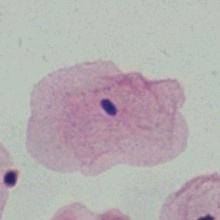
\includegraphics[width=0.3\textwidth]{194.jpg}}
\hspace{0.01\textwidth}
\subfigure[灰度图像]{\label{RGVFp1:b}
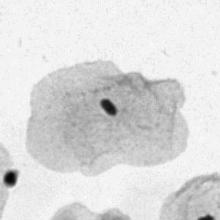
\includegraphics[width=0.3\textwidth]{194RGVFgray.jpg}}
\hspace{0.01\textwidth}
\subfigure[像素分类结果]{\label{RGVFp1:c}
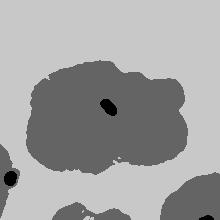
\includegraphics[width=0.3\textwidth]{194RGVFrough.jpg}}
\caption{原始图像、灰度图像、像素分类结果示意图}
\label{RGVFp1}
\end{figure}

接下来对降噪后的图像进行粗分割提取细胞质的初始轮廓。空间K均值方法可以将任意宫颈细胞灰度图像中的像素分为细胞核、细胞质、背景三类。用$(x,y)$表示像素点在图像中的位置,每个像素用三维特征向量$\vec{v}_{I}(x,y)$描述,

\begin{equation}
\vec{v}_{I}(x,y)=\left [ I(x,y),I_{mean}(x,y),I_{median}(x,y) \right ]
\label{RGVFv}
\end{equation}

其中$I(x,y)$表示该像素的灰度值,$I_{mean}(x,y)$、$I_{median}(x,y)$分别表示以当前像素为中心$5 \times 5$的窗口内像素的灰度平均值以及中值。在三维特征向量的基础上利用K-means算法将宫颈细胞图像的像素进行分类。图\ref{RGVFp1:c}为像素分类结果,统一设定分类后的细胞核区域的灰度值为0,细胞质区域的像素值为100,背景区域的像素值为200,观察可知像素分类后细胞质区域初步被提取出来,初始的Snake将被放置在像素分类结果的细胞质边界上。

像素分类后细胞质区域被提取出来作为细胞质分割的候选区域,同时提取出细胞核候选区域。然而细胞质区域内不仅包含当前细胞,还有相邻或重叠的其他细胞,算法将利用几何信息和灰度在细胞质候选区域的基础上提取出当前细胞区域进行后续分割,并提取出细胞核区域。一般情况下细胞质的面积大于细胞核的面积,因此算法依据细胞质区域和细胞核区域的面积设定阈值,进一步提取当前细胞的细胞质和细胞核。提取细胞质时,把面积最大的细胞质候选区域作为细胞质粗分割结果,并把该区域作为细胞核的搜索范围。提取细胞核时,结合像素分类结果在分割出的细胞质范围内提取面积最大的细胞核候选区域作为细胞核粗分割结果。此外,算法把候选区域中散落的面积较小的区域看作是噪声区域,粗分割时忽略了这些区域。

假设粗分割得到的细胞核区域包含$(x_{1},y_{1}),(x_{2},y_{2}),\cdots ,(x_{z},y_{z})$共z个像素点,$I(x,y)$为点$(x,y)$的在原始图像上的灰度值。细胞核的灰度值通常较小,为了避免除零细胞核的加权灰度值中心$(x_{c},y_{c})$计算方法为

\begin{equation}
%\left\{\begin{matrix}
x_{c}=\frac{\sum_{i=1}^{z}x_{i}(255-I(x_{i},y_{i}))}{\sum_{i=1}^{z}(255-I(x_{i},y_{i}))}\\ 
%y_{c}=\frac{\sum_{i=1}^{z}y_{i}(255-I(x_{i},y_{i}))}{\sum_{i=1}^{z}(255-I(x_{i},y_{i}))}
%\end{matrix}\right.
\label{RGVFcentroidx}
\end{equation}

\begin{equation}
y_{c}=\frac{\sum_{i=1}^{z}y_{i}(255-I(x_{i},y_{i}))}{\sum_{i=1}^{z}(255-I(x_{i},y_{i}))}
\label{RGVFcentroidy}
\end{equation}


Snake是一条连续的形状可控的曲线,$r(s)=(x(s),y(s)),s\in \left [ 0,1 \right ]$,其最小化能量函数为

\begin{equation}
E_{snake}=\int_{0}^{1}\left [ E_{int}(r(s))+E_{ext}(r(s)) \right ]ds
\label{ESnake}
\end{equation}

\begin{equation}
E_{int}(r(s))=\frac{\alpha \left | r_{s}(s) \right |^{2}+\beta \left | r_{ss}(s) \right |^{2}}{2}
\label{EintSnake}
\end{equation}
其中,$E_{int}(r(s))$为内部形变能量,也称内力,用来控制曲线的形状。而内力计算方法与传统的Snake算法相同,如式(\ref{EintSnake})。$E_{ext}(r(s))$为外部能量,又称外力,用来迫使曲线的形状向感兴趣区域的边界演化。传统的Snake算法对初始轮廓位置敏感,需要将初始Snake放置在感兴趣区域附近,而且在凹形轮廓处的收敛效果较差。Xu和Prince\cite{Xu1998Snakes}定义了梯度矢量流GVF,即$\vec{v}(x,y)=(u(x,y),v(x,y))$。同时,定义能量函数$E_{GVF}$为

\begin{equation}
E_{GVF}=\int\int \mu(u_{x}^{2}+u_{y}^{2}+v_{x}^{2}+v_{y}^{2})+\left | \bigtriangledown f \right |^{2}\left | \vec{v}- \bigtriangledown f\right |^{2}dxdy
\label{EGVF}
\end{equation}

式(\ref{EGVF})积分中第一项代表GVF平缓程度,第二项代表GVF与图像梯度的相似程度,$\mu$为权重系数,可控制两项对能量函数$E_{GVF}$的影响。$\bigtriangledown f=\left | \bigtriangledown I \right |$或者$f=\left | \bigtriangledown G_{\sigma } \ast  I \right |$,代表图像的梯度信息。

通过求解式(\ref{Euler})可得$\vec{v}(x,y)$的最优解,代入能量函数$E_{GVF}$求得Snake的外力$E_{ext}(r(s))$。$\bigtriangledown^{2}$是拉普拉斯算子。

\begin{equation}
\left\{\begin{matrix}
\mu \bigtriangledown _{u}^{2}-(u-f_{x})(f_{x}^{2}+f_{y}^{2})=0\\ 
\mu \bigtriangledown _{v}^{2}-(v-f_{x})(f_{x}^{2}+f_{y}^{2})=0
\end{matrix}\right.
\label{Euler}
\end{equation}

RGVF方法提出了图像的辐射边界图代替$E_{GVF}$中的$f$,以获取更好的分割效果。假设有一条辐射线段$l_{xb,yb}$从细胞核的加权灰度值中心$(x_{c},y_{c})$出发,经过细胞质边界上的点$(x_{b},y_{b})$,如图\ref{RGVFpLine}所示。

\begin{figure}[H]
\centering 
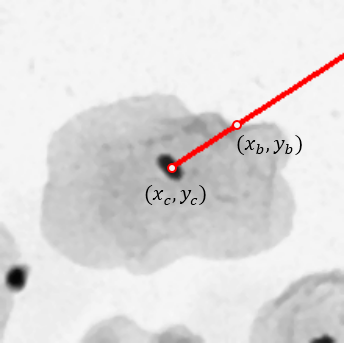
\includegraphics[width=0.3\textwidth]{lineRGVF.png}
\caption{辐射线示意图}
\label{RGVFpLine}
\end{figure}

则有$len_{cb}$表示从细胞核的加权灰度值中心$(x_{c},y_{c})$到细胞质边界上的点$(x_{b},y_{b})$的线段长度。若以细胞核加权灰度值中心为起始点增加辐射线段的数目,寻求每条辐射线段上属于细胞质边界的点即可得到细胞质的分割结果。

\begin{equation}
len_{cb}=\left \lfloor \sqrt{(x_{b}-x_{c})^{2}+(y_{b}-y_{c})^{2}} \right \rfloor
\label{lenb}
\end{equation}

定义线段$l_{xb,yb}$上某个点$x_{i},y_{i}$的辐射差$rd(x_{i},y_{i})$和点$x_{i},y_{i}$的辐射梯度$rg(x_{i},y_{i})$分别为

\begin{equation}
rd(x_{i},y_{i})=I(x_{i-1},y_{i-1})-I(x_{i},y_{i})
\label{rd}
\end{equation}

\begin{equation}
rg(x_{i},y_{i})=\frac{\left |rd(x_{i},y_{i})\right |+\left |rd(x_{i+1},y_{i+1}) \right |}{2}
\label{rg0}
\end{equation}

从细胞灰度图像可以看出,当沿着射线从细胞核的加权灰度值中心经过细胞质再到背景的像素,其灰度值越来越大。从辐射差计算公式(\ref{rd})可知从灰度值由小变大时的辐射差为负,细胞质边界点的辐射差应为负。在辐射线段上像素的辐射梯度在灰度变化明显的细胞核边界、细胞质边界和纹理或褶皱等位置都有较大的值,为了避免纹理或褶皱的影响,需要抑制辐射差为正的像素的辐射梯度值,抑制函数$F(x)$为

\begin{equation}
F(x)=\left\{\begin{matrix}
x &x< 0 \\ 
\gamma x & x\geq 0
\end{matrix}\right.
\label{Fx}
\end{equation}

抑制后的辐射梯度计算方法为

\begin{equation}
rg(x_{i},y_{i})=\frac{\left |F(rd(x_{i},y_{i}))\right |+\left |F(rd(x_{i+1},y_{i+1})) \right |}{2}
\label{rg}
\end{equation}

\begin{figure}[H]
\centering 
\subfigure[辐射线段灰度分布图]{\label{RGVFp2:a}
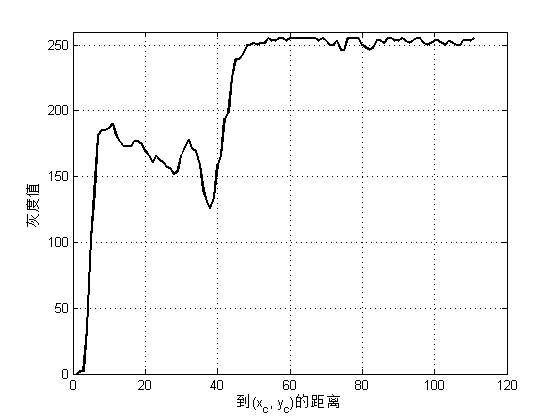
\includegraphics[width=0.45\textwidth]{line1.png}}
\hspace{0.001\textwidth}
\subfigure[辐射线段辐射差$rd$分布图]{\label{RGVFp2:b}
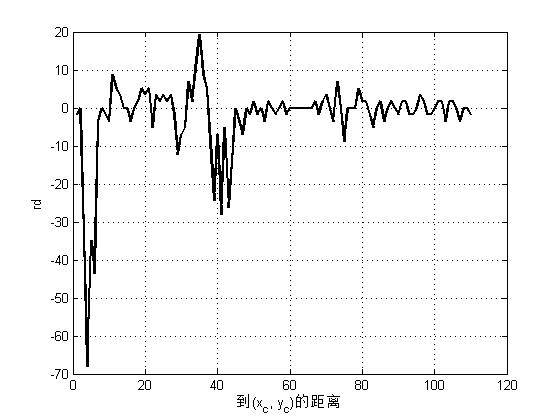
\includegraphics[width=0.45\textwidth]{line2.png}}
\vfill
\centering 
\subfigure[抑制前辐射梯度$rg$分布图]{\label{RGVFp2:c}
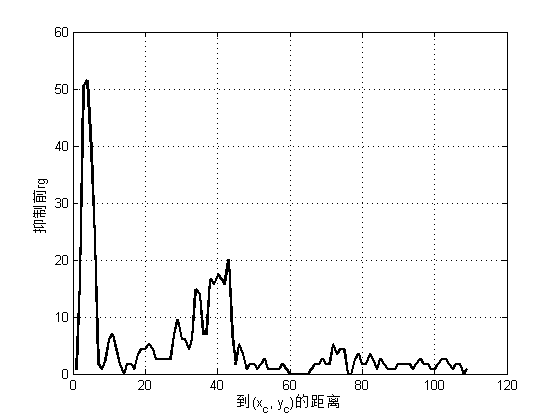
\includegraphics[width=0.45\textwidth]{line3.png}}
\hspace{0.001\textwidth}
\subfigure[抑制后辐射梯度$rg$分布图]{\label{RGVFp2:d}
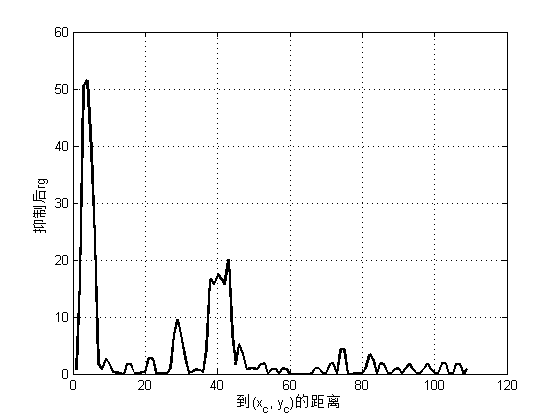
\includegraphics[width=0.45\textwidth]{line4.png}}
\caption{辐射线段上各点的灰度、辐射差$rd$、辐射梯度$rg$示意图}
\label{RGVFp2}
\end{figure}

图\ref{RGVFp2}展示了图\ref{RGVFpLine}中辐射线段上各点的灰度、辐射差$rd$、辐射梯度$rg$值的分布情况,这里$\gamma=0.1$,横坐标为辐射线段上各点到$(x_{c},y_{c})$的距离。观察图\ref{RGVFp2:a}可知,辐射线段上的灰度值在从细胞核到细胞质、从细胞质到背景的位置都明显增大。图\ref{RGVFp2:b}中辐射差$rd$在细胞核边界、细胞质强纹理或褶皱、细胞质边界附近的值为负,图\ref{RGVFp2:c}中抑制前辐射梯度$rg$在细胞核边界、细胞质强纹理或褶皱、细胞值边界附近的值较大。图\ref{RGVFp2:d}中抑制后辐射梯度$rg$明显削弱了辐射差为正位置相应的梯度值,表明抑制函数有效地降低了细胞质中的强纹理或褶皱对算法的影响。

然后基于辐射梯度生成辐射边缘图$MAP_{REM}$,代替$E_{GVF}$中的$f$,最终RGVF方法的能量函数为

\begin{equation}
E_{RGVF}=\int\int \mu(u_{x}^{2}+u_{y}^{2}+v_{x}^{2}+v_{y}^{2})+\left | \bigtriangledown MAP_{REM} \right |^{2}\left | \vec{v}- \bigtriangledown MAP_{REM}\right |^{2}dxdy
\label{ERGVF}
\end{equation}

\begin{figure}[H]
\centering 
\subfigure[辐射边界示意图]{\label{RGVFpic:a}
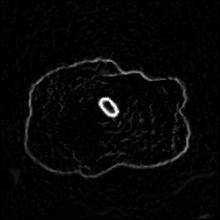
\includegraphics[width=0.3\textwidth]{194RGVFrem.jpg}}
\hspace{0.01\textwidth}
\subfigure[GVF示意图]{\label{RGVFpic:b}
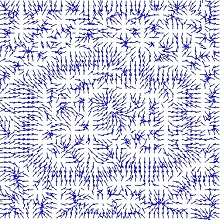
\includegraphics[width=0.3\textwidth]{194RGVFgvf.jpg}}
\hspace{0.01\textwidth}
\subfigure[RGVF方法结果]{\label{RGVFpic:c}
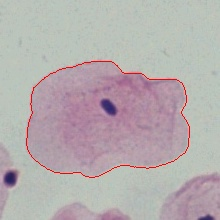
\includegraphics[width=0.3\textwidth]{194RGVFline.jpg}}
\caption{RGVF方法结果示意图}
\label{RGVFpic}
\end{figure}

图\ref{RGVFpic:a}为辐射边界图,能清晰的看到两条闭合的形状接近当前细胞细胞质和细胞核轮廓的白色曲线。图\ref{RGVFpic:b}为实验图像的GVF示意图,Snake曲线将在该外力的控制下向细胞质轮廓收敛。图\ref{RGVFpic:c}为RGVF方法的细胞质分割结果图,红色标记线即为细胞质边界,实验结果表明该算法对独立细胞的分割效果良好。

RGVF方法粗分割细胞核时,在像素分类后的细胞核待选区域中主要根据面积比例来提取当前细胞的细胞核,然而不同细胞的细胞核大小变化范围较大,该方法未能分割出部分实验图像的细胞核,实验过程中需手动标记细胞核加权灰度值中心以完成细胞的分割。该算法只适用于分割独立细胞,无法分割重叠细胞。

\section{水平集细胞分割方法}  

本节主要介绍Lu等人\cite{Lu2013Automated}结合水平集提出的自动分割重叠细胞的方法,该方法由两部分组成,首先要检测细胞簇和细胞核,然后结合水平集算法完成细胞分割。该方法的输入图像为灰度图像,原始图像和灰度图像分别如图\ref{Levels1:b}、图\ref{Levels1:b}所示。

检测细胞簇是为了提取出图像中的细胞区域,缩小细胞质分割的范围,便于进一步分割出每个细胞。通常情况下细胞核在细胞质内部,检测细胞核时限制检测范围为细胞簇内,因此细胞簇的分割也有助于缩小细胞核的检测范围。使用无监督的Quick shift算法\cite{Vedaldi2008Quick}将细胞图像进行超像素分割,考虑像素间的灰度值相似度和空间距离寻找局部最大值并对超像素分割结果进行标记。在标记后的图像上使用边缘检测器,检测出凸出的超像素边缘得到超像素边界图,同时有效地排除了大部分背景区域。利用无监督的二分类方法将图像分类为细胞和背景两部分。依据超像素分割结果绘制的凸包进行初始的细胞质分割,把凸包内的像素作为初始的细胞部分,凸包外的像素作为初始的背景部分,如图\ref{Levels1:c}中红色标记线所示。根据像素的灰度值,使用最大似然估计分别为细胞和背景学习高斯混合模型,进一步提取细胞质部分,结果如图\ref{Levels1:d}中红色标记线所示。

假设图像中的细胞核没有重叠情况,每个细胞核代表一个细胞,细胞核的分割是该算法的关键步骤。细胞核有相对较低的灰度值、颜色均匀等特点,且形状大多近似圆形。MSER算法\cite{Matas2004Robust}利用像素灰度值和邻近程度判断像素连通情况,可以初步检测出图像中分类为细胞部分区域内的细胞核,之后计算检测出细胞核的离心率,忽略离心率较大即形状与圆形偏差较大的细胞核,得到细胞核分割结果。当前细胞的细胞核如图\ref{Levels1:e}中绿色标记线所示。

\begin{figure}[H]
\centering 
\subfigure[原始图像]{\label{Levels1:a}
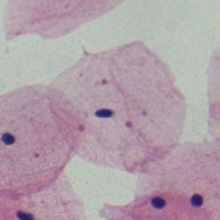
\includegraphics[width=0.3\textwidth]{12.jpg}}
\hspace{0.01\textwidth}
\subfigure[灰度图像]{\label{Levels1:b}
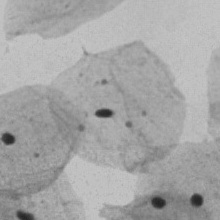
\includegraphics[width=0.3\textwidth]{12g.jpg}}
\hspace{0.01\textwidth}
\subfigure[凸包示意图]{\label{Levels1:c}
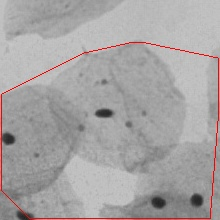
\includegraphics[width=0.3\textwidth]{RawRet.jpg}}
\vfill
\centering 
\subfigure[细胞质部分]{\label{Levels1:d}
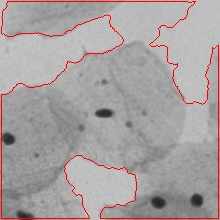
\includegraphics[width=0.3\textwidth]{RefinedRet.jpg}}
\hspace{0.01\textwidth}
\subfigure[细胞核]{\label{Levels1:e}
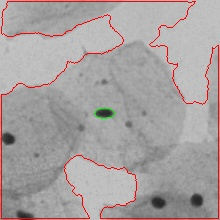
\includegraphics[width=0.3\textwidth]{NuRet.jpg}}
\caption{水平集细胞分割方法示意图}
\label{Levels1}
\end{figure}

水平集方法主要依据细胞核的个数对细胞质部分进行分割,把细胞质部分分割为与细胞核数目相等的细胞。把细胞质的初步分割结果如图\ref{Levels1:d}中红色标记线作为水平集函数的初始值,在能量函数的控制下完成细胞分割。

接下来主要介绍水平集方法。水平集方法\cite{Osher1988Fronts}的思想是将曲线用一个曲面的零水平集来表示,并通过曲面的演化使得对应曲线贴合目标的边缘。曲面$\phi (t,x,y)$的零水平集$C(t)$表示曲面与平面$z=0$的交线:

\begin{equation}
C(t)=\left \{ (x,y)| \phi (t,x,y)=0  \right \}
\end{equation}

而曲面的演化规则为:

\begin{equation}
\frac{\partial \phi }{\partial t}+F\left | \bigtriangledown \phi \right |=0
\label{lvlseteq}
\end{equation}

式(\ref{lvlseteq})也被称为水平集方程,其中$F$可以控制曲面演化,被称为速度方程。传统的水平集求解方法在迭代过程中要求水平集函数近似为一个符号距离函数(Signed Distance Function),即要求$\left | \bigtriangledown \phi \right |=1$。
为了满足这个条件,在迭代中不得不周期性地重新初始化水平集函数,该过程不仅速度慢,而且影响后续计算结果的准确性。由于传统的水平集演化方法存在以上问题,现在更常用的是Li等人\cite{Li2005Level}提出的另一种方法,通过最小化一个能量函数$\varepsilon(\phi )$来迭代水平集函数:

\begin{equation}
\varepsilon (\phi )=\mu P(\phi )+\varepsilon_{m} (\phi )
\label{engfunc}
\end{equation}



其中$\varepsilon_{m}(\phi )$是一个与图像相关的能量函数,能控制零水平集的移动,在不同的使用场景下有不同的定义,而$P(\phi )$是一个约束项,它使得水平集函数不能偏离符号距离函数太远。

\begin{equation}
P(\phi )=\int_{\Omega }\frac{1}{2}(|\bigtriangledown \phi |-1)^{2}d\mathbf{x}
\end{equation}

水平集演化方程定义为

\begin{equation}
\frac{\partial \phi }{\partial t}=-\frac{\partial \varepsilon }{\partial \phi }
\label{lvlseteqt}
\end{equation}

使用这个约束后,水平集演化过程中无须再进行重新初始化,不仅提高了算法的效率,也使得算法更加稳健。式(\ref{engfunc})中能量函数可以有不同的定义方式,Lu等人\cite{Lu2013Automated}提出了一种用于宫颈细胞分割的能量函数:


\begin{equation}
\varepsilon _{u}(\phi)=\mu R({\phi})+\lambda L({\phi})+\alpha A({\phi})+\rho P_{p}({\phi})+\varepsilon _{b}(\phi)
\label{LevelSetEu}
\end{equation}

其中$L(\phi)$衡量零水平集的长度,即细胞边缘的长度,而$A(\phi)$衡量分割得到前景区域的面积,$P_{p}({\phi})$是前景的形状先验项,$\varepsilon _{b}(\phi)$为优化项,参数$\mu>0$,$\lambda>0$,$\alpha$,$\rho$为任意实数。
\begin{equation}
R(\phi  )=P(\phi   )
\end{equation}

\begin{equation}
L(\phi  )=\int_{\Omega }g\delta (\phi  )|\bigtriangledown \phi  |d\mathbf{x}
\end{equation}

\begin{equation}
A(\phi  )=\int_{\Omega }gH (-\phi  )d\mathbf{x}
\end{equation}

\begin{equation}
P_{p}({\phi})=\int_{\Omega }gH(-p({\phi}))d\mathbf{x}
\end{equation}

其中$g=\frac{1}{1+ \left | G_{\sigma }\ast I \right |}$,$G_{\sigma }$是标准差为$\sigma$高斯核,$H(\cdot )$为Heaviside函数,$p({\phi})$表示水平集函数估计的椭圆形状,


基于该能量函数定义进行优化,使用式(\ref{lvlseteqt})进行水平集演化一定次数后,最终得到的零水平集被认为是细胞质的边界,文献\citen{Lu2013Automated}中指出该方法对于巴氏染色的宫颈细胞图像有较好效果,本文在Feulgen和伊红染色的宫颈细胞图像上进行实验该方法仍可以取得良好的分割效果。图\ref{Levels2}为水平集细胞分割方法分割结果,红色标记线表示当前细胞的细胞质边界。

\begin{figure}[H]
\centering 
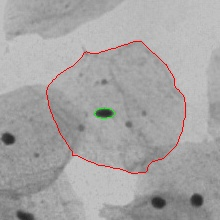
\includegraphics[width=0.3\textwidth]{LSret.jpg}
\caption{分割结果示意图}
\label{Levels2}
\end{figure}


\begin{figure}[H]
\centering 
\subfigure[]{\label{Levels3:a}
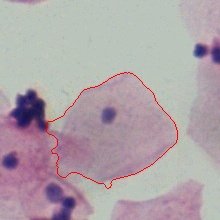
\includegraphics[width=0.3\textwidth]{2lsline.jpg}}
\hspace{0.01\textwidth}
\subfigure[]{\label{Levels3:b}
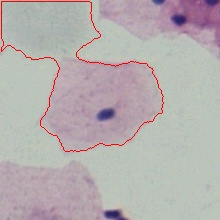
\includegraphics[width=0.3\textwidth]{52lsline.jpg}}
\hspace{0.01\textwidth}
\subfigure[]{\label{Levels3:c}
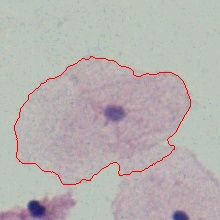
\includegraphics[width=0.3\textwidth]{57lsline.jpg}}
\caption{水平集方法的细胞质分割结果}
\label{Levels3}
\end{figure}
水平集方法对部分实验图像的细胞质分割结果如图\ref{Levels3}所示。图\ref{Levels3:a}中分割结果受炎症细胞的干扰,分割结果呈锯齿状,图\ref{Levels3:b}中图像左上角的阴影区影响了分割结果,错误地将阴影区分割为细胞,图\ref{Levels3:c}中未能准确分割出当前细胞与其他细胞的重叠部分,将其他细胞的细胞质分割为当前细胞。
\section{本章小结}
本章主要介绍了适用于分割独立细胞的RGVF方法和用于分割独立细胞和重叠细胞的水平集方法,详细地介绍了两种方法的基本原理,并进行实验分析。实验结果表明RGVF方法对独立细胞的分割结果良好,水平集方法对独立细胞和重叠细胞的分割结果良好。

\chapter{最小代价路径算法}  
\section{引言}     
细胞分割是细胞病理分析和分类的关键点和难点,特别是多个细胞重叠情况下细胞质的分割一直都是国内外专家学者研究的热点问题。Feulgen染色主要用于DNA定量测定,染色后的细胞核呈紫色,该染色法仅对样本的细胞核部分进行染色,细胞质部分则不染色。H-E染色法,俗称苏木精——伊红染色法,其中苏木精将细胞核染成鲜明的蓝色,而伊红将细胞质染成不同深浅的粉红色至桃红色。该方法染色步骤简单,染色液渗透性强,染色后细胞的透明度好、细胞核和细胞质对比明显,效果稳定。采用Feulgen染色和伊红染色复合染色后宫颈细胞的细胞核呈蓝紫色,细胞质呈桃红色。本文所研究的细胞质分割算法的实验图像将染色后宫颈细胞制备成刮片,然后进行扫描获取的显微图像。如图\ref{part}所示。

\begin{figure}[H]
\centering
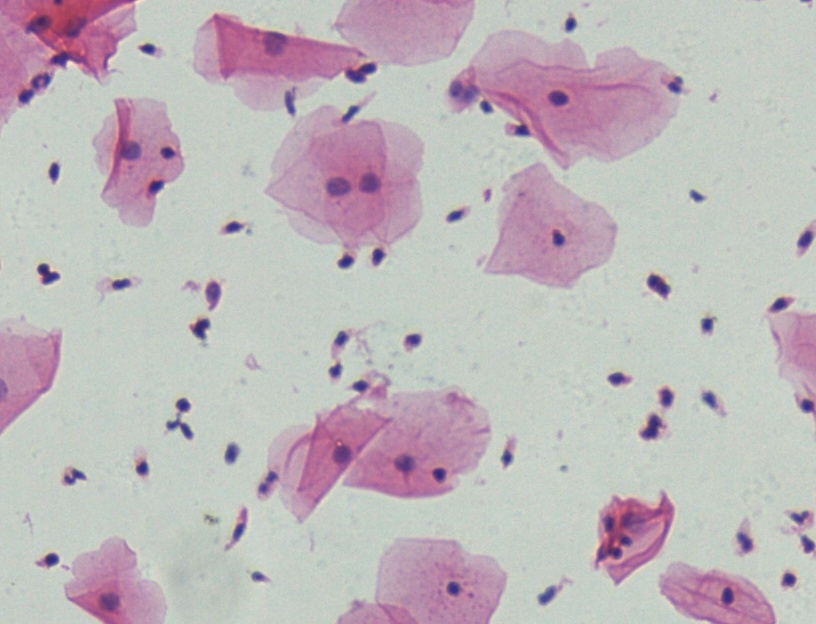
\includegraphics[width=0.7\textwidth]{part.jpg}
\caption{扫描获取的局部宫颈细胞示意图\label{part}}
\end{figure}

影响细胞质分割的因素有很多,其中主要包括:染色制片后宫颈细胞的形态多样性,细胞质内部包含丰富的纹理和褶皱;染色工艺造成的细胞质部分染色不均匀现象;多个细胞之间存在不同程度的相互重叠;图像中普遍存在诸如粘液、炎症细胞、血细胞等杂质;图像采集设备成像效果不稳定以及成像过程中包含的噪声等。这些问题对细胞质边界的分割造成一定程度的干扰,给分割带来了很大的难度。实际采集的宫颈细胞图像中有独立的单个细胞,通常情况下细胞重叠的现象也很多,如图\ref{part}。

考虑到这些因素,本文提出了一种自动分割重叠细胞的算法,根据染色后细胞核、细胞质、背景在RGB颜色通道的差异,首先对图像进行极坐标变换,通过将图像从笛卡尔坐标系转换到极坐标系下进行采样获得采样矩阵,这里利用采样点计算得到的梯度信息经过转换函数生成代价矩阵,并考虑细胞核周围附近的高亮区域、背景区域等对分割结果的影响添加约束条件对代价矩阵进行优化,用全局最优的方法求取最小代价路径来获取细胞的边界。

\subsection{获取采样图像}
相比颜色深浅不一、形状多变的细胞质区域,宫颈细胞细胞核的形状较为规则、颜色比较均一,因此是定位细胞的一个良好标志。本文研究的样本图像,前期使用细胞核分割方法获取了细胞核的位置,然后以细胞核为中心,提取完整的细胞区域。通过观察比对大量实验数据,考虑到图像中需包含独立细胞或多个细胞的情况,提取大小为220$\times$220像素的图像作为实验图像。

由于图像在成像过程中不可避免的会受到噪声的污染,为防止噪声对细胞质分割造成干扰须对图像做降噪处理。高斯滤波主要用与处理服从正态分布的噪声,处理细胞图像时容易产生细胞边界的模糊。平滑线性空间滤波器,又称为均值滤波器,主要用于去除比滤波器尺寸较小的噪声区域。中值滤波一种非线性平滑滤波技术,在去除噪声的同时能较好保护图像边缘细节,对处理脉冲噪声非常有效。中值滤波器是一种经典的降噪方法,比同尺寸的线性平滑滤波器的模糊程度明显要低。

Bilateral滤波\cite{Tomasi1998Bilateral},也叫双边滤波,同时考虑了像素的空间距离和像素值两个因素,具有降噪的同时保持边界的特性。但在纹理较强的区域滤波效果较差,且计算速度较慢。若用$f_{in}(x,y)$表示待处理的图像,$f_{o}(x,y)$表示滤波后的图像,$A_{x,y}$表示以$(x,y)$为中心大小为$n\times n$($n$为奇数)的邻域范围,则有

\begin{equation}
f_{o}(x,y)=\frac{\sum\limits_{(i,j)\in A_{x,y}}w(i,j)f_{in}(i,j)}{\sum\limits_{(i,j)\in A_{x,y}}w(i,j)}
\label{BilateralEq}
\end{equation}

式(\ref{BilateralEq})中$w(i,j)$为加权系数,是距离因子$w_{d}(i,j)$和亮度因子$w_{i}(i,j)$两部分的乘积,参数$\sigma _{d}$和$\sigma _{i}$可以分别调整距离因子和亮度因子的值。

\begin{equation}
w(i,j)=w_{d}(i,j)w_{i}(i,j)
\label{BilateralW}
\end{equation}

\begin{equation}
w_{d}(i,j)=exp\left ( -\frac{(i-x)^{2}+(j-y)^{2}}{2\sigma _{d}^{2}} \right )
\label{BilateralWd}
\end{equation}

\begin{equation}
w_{i}(i,j)=exp\left ( -\frac{\left | f_{in}(i,j)-f_{in}(x,y) \right |^{2}}{2\sigma _{i}^{2}} \right )
\label{BilateralWi}
\end{equation}

第二章中的RGVF细胞分割方法使用的非局部均值滤波方法速度较慢,对算法运行时间影响较大,本文不使用该方法滤波。为了使本文提出的算法具有较快的速度将选择一种速度较快的滤波方法,并运用到所有细胞分割的实验中便于对比分析各方法的运行时间。不同滤波方法的效果对比如图\ref{filterret}所示,其中图\ref{filter:a}为原始图像,图\ref{filter:b}为高斯滤波结果,图\ref{filter:c}为$3\times 3$模板下的均值滤波结果,图\ref{filter:d}为$3\times 3$模板下的中值滤波结果,图\ref{filter:e}为双边滤波效果。观察实验结果可知,高斯滤波结果图像明显地被模糊了,中值滤波结果相比比均值滤波结果和双边滤波结果边界保持较好。而双边滤波的运行速度较慢,会增加算法的运行速度。通过分析对比发现中值滤波最适合做分割前的滤波,因此本文采用了中值滤波对图像进行滤波处理。

\begin{figure}[H]
\centering 
\subfigure[原始图像]{\label{filter:a}
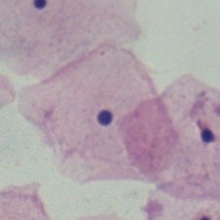
\includegraphics[width=0.3\textwidth]{107.jpg}}
\hspace{0.01\textwidth}
\subfigure[高斯滤波结果]{\label{filter:b}
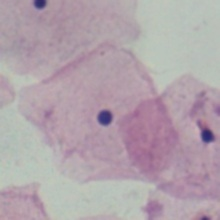
\includegraphics[width=0.3\textwidth]{G107.jpg}}
\hspace{0.01\textwidth}
\subfigure[均值滤波结果]{\label{filter:c}
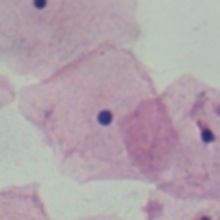
\includegraphics[width=0.3\textwidth]{j107.jpg}}
\vfill
\centering 
\subfigure[中值滤波结果]{\label{filter:d}
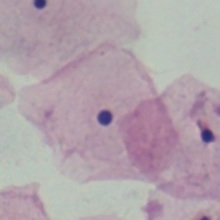
\includegraphics[width=0.3\textwidth]{z107.jpg}}
\hspace{0.01\textwidth}
\subfigure[双边滤波结果]{\label{filter:e}
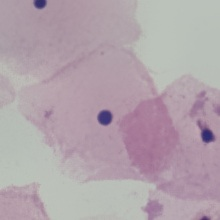
\includegraphics[width=0.3\textwidth]{s107.jpg}}
\caption{滤波方法结果对比图}
\label{filterret}
\end{figure}


\subsection{建立采样模型}
从细胞样本图像中可以看出,细胞质环绕分布在细胞核周围,形状不规则但边界较为平滑,因此可以把细胞质的边界看作是一条围绕细胞核的封闭曲线。通常情况下,图像都以笛卡尔坐标系的方式显示,而采用极坐标\cite{Xu2013Cell}的方式可以把细胞质的分割问题转换为寻求一条围绕极坐标原点的闭合曲线,可以减小计算量更有利于实现处理。


采用极坐标表示图像,坐标系的原点位于细胞核内,细胞质的边界即为一系列围绕原点连续分布的像素点。本文算法将使用极坐标系分析图像,将二维图像通过极坐标变换进行处理。建立的采样模型以图像中心为起点,在相等间隔角度均匀向外辐射的线段上进行等间距采样,每条线段表示一个采样方向。最终通过对这些采样点的计算处理获取细胞质的边界。假设每个采样方向上的采样点中有且只有一个采样点恰好处于细胞质的边界上,这些不同方向上位于细胞质边界的一组采样点围绕成的闭合曲线就组成了细胞质的边界,即该闭合曲线即为细胞质的分割结果。如果采样点越密集,则组成的闭合曲线越平滑,分割结果越准确越接近真实的细胞质边界。

\begin{figure}[H]
\centering 
\subfigure[极坐标采样模型]{\label{Samppoint:a}
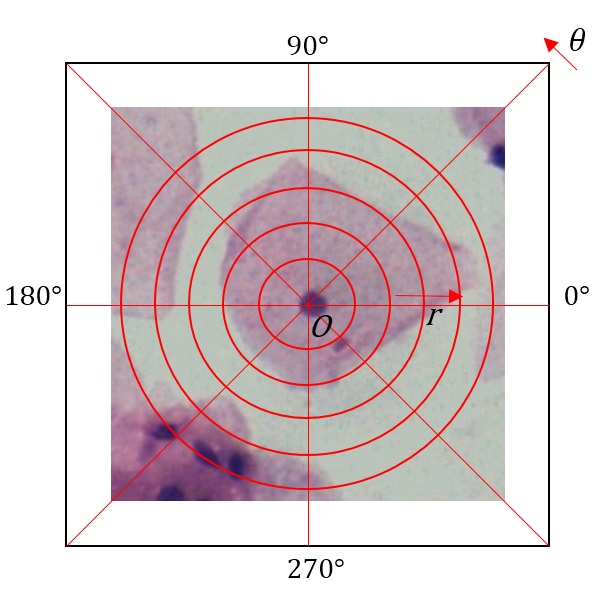
\includegraphics[width=0.46\textwidth]{Samp.jpg}}
\hspace{0.001\textwidth}
\subfigure[采样点示意图]{\label{Samppoint:b}
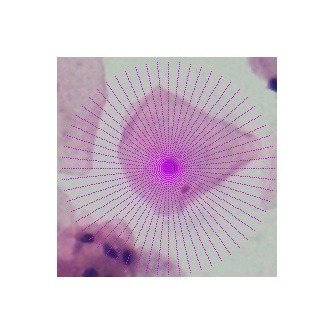
\includegraphics[width=0.46\textwidth]{Samppoint1.jpg}}
\centering 
\subfigure[极坐标下细胞图像展开示意图]{\label{Samppoint:c}
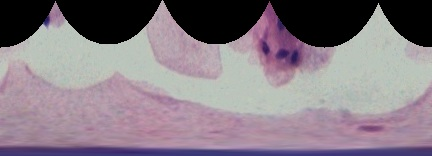
\includegraphics[width=0.7\textwidth]{po.jpg}}
\caption{采样模型示意图}
\label{Samppoint}
\end{figure}

这里设图像的中心为极坐标的原点$O$,如图\ref{Samppoint:a}所示,极坐标系中每个像素点的位置用$(r_{i},\theta_{j} )$表示,其中$r$表示模,$\theta$表示角度。这里用$M$表示采样方向的数目,$N$表示每个采样方向上采样点的数目,则采样点的极坐标$(r_{i},\theta_{j} )$计算法方法为:

\begin{equation}
r_{i}=\frac{i}{N}len\left ( 0\leqslant i < N \right )
\label{r}
\end{equation}

\begin{equation}
\theta _{j}=\frac{2\pi j}{M} \left ( 0\leqslant j< M \right )
\label{theta}
\end{equation}

其中,$len$表示采样线段的长度,大小为图像高度和宽度较小值的一半。


在样本图像上以图像的中心点作为起始点,绘制$M=60$个采样方向,每个采样方向等间隔地分布$N=60$个采样点,则相邻两个采样方向的夹角为:

\begin{equation}
\Delta \theta=\frac{2\pi}{M} 
\label{_theta}
\end{equation}

综上所述,建立的采样模型如图\ref{Samppoint:b}所示。

由极坐标系计算图像中采样点的位置方法如下:
\begin{equation}
x=r_{i}cos\theta _{j}+\frac{1}{2}width
\label{x}
\end{equation}

\begin{equation}
y=r_{i}sin\theta _{j}+\frac{1}{2}height
\label{y}
\end{equation}

$width$为图像的宽度,$height$为图像的高度,图\ref{Samppoint:b}中每一个紫色点表示相应采样点的位置$(x,y)$。图\ref{Samppoint:c}是极坐标下细胞图像展开示意图,当前细胞的细胞核在图中底部位置。为了实现算法将把样本图像的采样点再从极坐标转换到笛卡尔坐标系下,用采样点建立二维矩阵$S$,矩阵大小为$M\times N$。从细胞图像中可以明显看出细胞质部分呈粉红或桃红色,在分析了细胞图像中细胞质、细胞核、背景等部分各颜色通道值的特点之后发现细胞质区域像素的红色通道与绿色通道的差与其他区域有明显的区别,可作为区分细胞质区域与非细胞质区域的依据,因此采样矩阵中记录的值是细胞图像中采样点位置红色通道与绿色通道差。采样矩阵$S$表示如下:

\begin{equation}
S=\begin{bmatrix}
S_{0,0} & S_{0,1} &  \cdots & S_{0,N-1}\\ 
S_{1,0} &  \vdots &  \ddots & \vdots\\ 
 \vdots &  \vdots &  \ddots & \vdots \\ 
S_{M-1,0} &  \cdots &  \cdots & S_{M-1,N-1}
\end{bmatrix}
\label{S}
\end{equation}

用$RG$表示由彩色图像红色通道与绿色通道差计算得到的图像,采样矩阵$S$中每个采样点记录的值表示为:

\begin{equation}
S_{j,i}=RG_{r_{i}cos\theta _{j}+\frac{1}{2}width,r_{i}sin\theta _{j}+\frac{1}{2}height}
\label{PtoI}
\end{equation}

\section{最小代价路径算法实现}

最小代价路径算法实现是在代价矩阵上进行全局搜索实现的。在得到采样矩阵之后,通过对每个采样点计算梯度、使用代价转换函数计算每个采样点的代价值进而得到代价矩阵。

\subsection{计算代价矩阵}
每个采样点都可能是细胞质边界的路径点,用代价表示这个可能性,代价值越小则该点成为细胞质边界的可能性越大,代价值越大则相反。首先定义代价矩阵为Cost,大小为$M\times N$与采样矩阵相同。

\begin{equation}
Cost=\begin{bmatrix}
Cost_{0,0} & Cost_{0,1} &  \cdots & Cost_{0,N-1}\\ 
Cost_{1,0} &  \vdots &  \ddots & \vdots\\ 
 \vdots &  \vdots &  \ddots & \vdots \\ 
Cost_{M-1,0} &  \cdots &  \cdots & Cost_{M-1,N-1}
\end{bmatrix}
\label{COST}
\end{equation}

为保证计算结果的准确,本文算法初始化代价矩阵所有元素的值为0,表示当前的采样点中不存在组成细胞质边界的路径点,即
\begin{equation}
Cost_{i,j}=0
\label{cost0}
\end{equation}

然后在每条采样线段上遍历采样点,并计算该点的梯度。为了抑制内部纹理的影响,用同一采样方向上的相邻的四个采样点$S_{i,j-1}$、$S_{i,j-2}$、$S_{i,j+1}$、$S_{i,j+2}$计算采样点$S_{i,j}$的梯度,梯度计算方法为:

\begin{equation}
\bigtriangledown S_{i,j}=S_{i,j-1}-S_{i,j-2}-S_{i,j+1}+S_{i,j+2}(2<j<N-2)
\label{gradient}
\end{equation}

接下来对梯度矩阵$\bigtriangledown S$做变换得到代价矩阵Cost。梯度值越大,表示该点与采样线段上前后相邻像素的颜色变化越明显,该点成为边界的可能性越大。由梯度值计算代价的转换函数为:

\begin{equation}
Cost_{i,j}=exp\left ( -a\bigtriangledown S_{i,j} \right ) \quad  \left ( a\in R^{+} \right )
\label{cost}
\end{equation}

$a$是参数,本章取$a$为0.14。该转换函数可以将较大的梯度值转换为较小的代价值。

\begin{figure}[H]
\centering
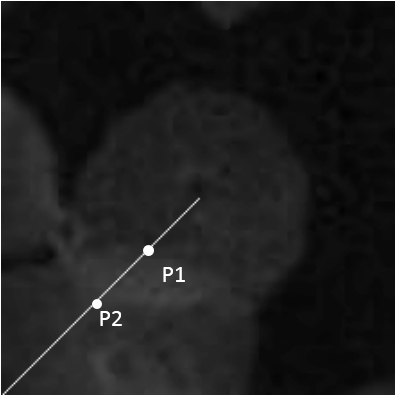
\includegraphics[width=0.3\textwidth]{155RGLine.png}
\caption{代价值说明图\label{RGcost}}
\end{figure}

如图\ref{RGcost}所示为由彩色图像红色通道与绿色通道差计算得到的图像,点$P1$、$P2$为采样线段上的两个点。采用式(\ref{gradient})计算出的点$P1$的梯度值为负,转换后的代价值较大,点$P2$的梯度值为正,得到的代价值较小,因此点$P2$成为边界的可能性大于点$P1$,从而可以有效地处理细胞质重叠部分的分割。

对代价矩阵中每个采样方向上采样点的代价值即每行数据分别进行归一化处理,得到用于计算最小代价路径的代价矩阵。

\begin{equation}
Cost_{i,j}=\frac{Cost_{i,j}}{\sum\limits_{j=0}^{N}Cost_{i,j}}
\label{norcost}
\end{equation}

最后,将采样矩阵中前两列和最后两列点的值设为较大的值,如9999等表示其代价很大,这些点的位置在细胞核内或者靠近图像边缘成为边界的可能性很小。

\subsection{搜索最小代价路径}

定义一条闭合路径为从采样矩阵第0行的任意点为起始点出发,经过第$1,2,...,M-1$行中的任意点并回到该起始点所经过的采样点组合。每个采样点在代价矩阵中都有相应的代价值,代价矩阵中某点的值越小,表示该点成为边界的可能性越大。最小代价路径是所有可能的闭合路径中采样点代价和最小的路径点组合。

由于每条路径的起始点都是采样矩阵的第0行中的一点,一条闭合路径必然会依次经过第$1,2,...,M-1$行中的点,相邻两点的列坐标差越大表示该路径代表的边界越陡峭。又因为大多数细胞的边界是平滑的,因此这里一方面仅允许相邻两点列坐标相差不超过5,另一方面根据列坐标的差异适当地增加惩罚,使得最终得到的路径点连续且平滑,避免了细胞质分割结果产生过于陡峭的边界。惩罚函数为$W(d)$,d表示相邻两点列坐标的差值。d的绝对值越大表示相邻两点在图像上的位置距离越远,相邻两点成为同一路径上相邻边界点的可能性越小,相应的惩罚系数值应当越大,因此参数之间的关系为$ 1.0<\alpha<\beta<\gamma<\eta<\omega<  +\infty$。

\begin{equation}
W(d)=\left\{\begin{matrix}
1.0 & d = 0\\ 
 \alpha & d=\pm 1\\ 
\beta  & d=\pm 2\\ 
 \gamma & d=\pm 3\\ 
 \eta & d=\pm 4\\ 
 \omega & d=\pm 5\\ 
 +\infty & otherwise
\end{matrix}\right.
\label{W}
\end{equation}

在搜索过程中,定义了路径矩阵R、累计代价矩阵$SumCost$。因为路径是闭合的,为方便计算在代价矩阵第$M-1$行后添加第0行的一个副本作为第M行数据。每条搜索路径的起始点为第0个采样方向上的采样点$S_{0,k}(k\in [0,N-1])$,因此共搜索N条路径。累计代价矩阵$SumCost$的大小为$(M+1)\times N$,用来记录以当前起始点搜索到第$(i,j)$个采样点的最优路径上所有采样点的代价总和。每次从不同的起始点搜索路径前,必须初始化累计代价矩阵$SumCost$的每个元素为无穷大,表明当前不存在任何路径。路径矩阵R大小为$(M+1)\times N$,用来记录采样点$S_{i,j}$所在最小代价路径的前一个点$S_{i-1,m}$($m$与$j$的差满足d的范围)的位置,$R_{i,j}=m$。累计代价矩阵$SumCost$、路径矩阵R表示为:

\begin{equation}
SumCost=\begin{bmatrix}
SumCost{0,0} & SumCost{0,1} &  \cdots & SumCost{0,N-1}\\ 
SumCost{1,0} &  \vdots &  \ddots & \vdots\\ 
 \vdots &  \vdots &  \ddots & \vdots \\ 
SumCost{M-1,0} &  \vdots &  \ddots & SumCost{M-1,N-1}\\
SumCost{M,0} &  \cdots &  \cdots & SumCost{M,N-1}
\end{bmatrix}
\label{SumCost}
\end{equation}

\begin{equation}
R=\begin{bmatrix}
R_{0,0} & R_{0,1} &  \cdots & R_{0,N-1}\\ 
R_{1,0} &  \vdots &  \ddots & \vdots\\ 
 \vdots &  \vdots &  \ddots & \vdots \\ 
R_{M-1,0} &  \vdots &  \ddots & R_{M-1,N-1}\\
R_{M,0} &  \cdots &  \cdots & R_{M,N-1}
\end{bmatrix}
\label{R}
\end{equation}



每次搜索路径的起始为点采样矩阵的第0行中的一点,假设当前搜索路径的起始点为$S_{0,k}$,则该采样点的代价表示为$Cost_{0,k}$。点$S_{0,k}$作为搜索路径的第一个点它的代价将直接赋值给累计代价矩阵中的元素$SumCost_{0,k}$,即

\begin{equation}
SumCost_{0,k}=Cost_{0,k}
\label{Sum0}
\end{equation}

下一步搜索第1个采样方向上的采样点$S_{1,j}$。为了使最终的路径连续且平滑使用惩罚函数(\ref{W})作为采样点$S_{1,j}$相应代价的系数进行累加,只对满足参数d条件的采样点进行计算。

\begin{equation}
SumCost_{1,j}=SumCost_{0,k}+W(k-j)Cost_{1,j}
\label{Sum1}
\end{equation}

当搜索到第2个采样方向上的采样点$S_{2,j}$时,路径可通过第1个采样方向上多个采样点搜索到达$S_{2,j}$,须进行比较选择搜索从$S_{0,k}$出发经过$S_{1,m}$到达$S_{2,j}$代价和最小值作为累计代价矩阵元素$SumCost_{2,j}$的值。同时记录路径矩阵$R[2,j]$为$m$,表示到达$S_{2,j}$的最小代价路径经过点$S_{1,m}$。

\begin{equation}
SumCost_{2,j}=\min \left ( SumCost_{1,m}+W(m-j)Cost_{2,j} \right )
\label{Sum2}
\end{equation}

之后的搜索的采样点计算方法类似式(\ref{Sum2}),每次计算$SumCost_{i,j}$后都与先前记录的值进行比较,取较小的值更新记录,同时在R中记录下搜索到当前点时经过的上一个点的列坐标。以$S_{0,k}$为起始搜索点的路径,其终点必然是$S_{M,k}$。路径总代价$PathCost$表示全局搜索得到的一条完整闭合路径的总代价,最终大小由N条路径搜索完成后取最小值,就是要寻求的最小代价路径上个路径点的代价值之和。

\begin{equation}
PathCost=\min_{0\leqslant k < N} \left ( SumCost_{M,k} \right )
\label{PathCost}
\end{equation}

以$S_{0,k}$为起始搜索点的路径搜索结束后得到一条路径,可通过路径矩阵$R$遍历该路径上的每一个点即组成最小代价路径的采样点。路径矩阵中$R_{i,j}$的值为表示最小代价路径经过第$i-1$个采样方向上的路径点的列坐标,说明第$i-1$个采样方向上的路径点为$S_{i-1,R_{i,j}}$。一条完整的路径有M个路径点,因此定义路径为一维数组$Road[M]$依次记录各采样方向上路径点的列坐标。要注意的是,当$i=0$时第0个采样方向上的路径点可根据当前计算得到的最小的路径总代价$PathCost$的起始点直接给出,即路径点为$S_{0,k}$,故有
\begin{equation}
Road_{0}=k
\label{Road0}
\end{equation}

每次路径搜索结束后,把$S_{M,k}$也作为路径的第0个路径点等同于$S_{0,k}$,第$M-1$个路径点表示第$M-1$个采样方向上的路径点,则其列坐标记录在$R_{M,k}$中,其列坐标计算方法为
\begin{equation}
Road_{M-1}=R_{M,Road_{0}}
\label{Road1}
\end{equation}

可得计算路径点的递推关系式(\ref{Roadi}),通过递推关系可知属于最小代价路径的全部路径点的位置,每个路径点表示为$S_{i,Road_{i}}$。
\begin{equation}
Road_{i}=R_{i+1,Road_{i+1}}(1\leq i\leq M-2)
\label{Roadi}
\end{equation}

通过对不同起始点搜索得到的所有路径比较得到最小的路径总代价$PathCost$,推导出该路径上的路径点即是最小代价路径,把路径点绘制到细胞图像中即可得到细胞质的分割结果。

定义$MCP(S_{0,k},\cdots ,S_{M,k})$为以第0行第k个采样点作为起始点出发开始搜索直至到达第M行第k列采样点的最小代价路径,包含了最小代价路径上各路径点。则路径有如下状态转移方程:
 
%  \begin{equation}
% \begin{aligned}
%  MCP(S_{0,k},\cdots ,S_{M-1,k})&= \\ 
%  &\min_{0\leqslant k < N}\left \{ MCP(S_{0,k},\cdots ,S_{i,j})+MCP(S_{i,j},\cdots ,S_{M-1,k}) \right \} 
% \end{aligned}
% \end{equation}

\begin{equation}
MCP(S_{0,k},\cdots ,S_{M-1,k})=\min_{0\leqslant k < N}\left \{ MCP(S_{0,k},\cdots ,S_{i,j})+MCP(S_{i,j},\cdots ,S_{M-1,k}) \right \}
\label{MCPk}
\end{equation}

推广到一般情况,以采样点$S_{0,k}$为起始点的路径经过$S_{i-1,m}$到达采样点$S_{i,j}$的最小代价路径可表示为

\begin{equation}
 MCP(S_{0,k},\cdots ,S_{i-1,m})+ W(m-j)Cost_{i,j}
\label{MCPnext}
\end{equation}

综上所述,全局的最小代价路径$MCP$可以表示为:

\begin{equation}
MCP =\min_{0\leqslant k < N}\left \{ MCP(S_{0,k},\cdots ,S_{M-1,k}) \right \}
\label{MCP}
\end{equation}

这里总结了最小代价路径算法的具体步骤,该算法对细胞图像进行全局搜索最小代价路径的过程如下: 

\begin{algorithm}[H]
\caption{\label{minpathalgdescp}最小代价路径算法}
\begin{algorithmic}[1]
\STATE 计算各采样方向上的采样点坐标$S_{i,j}$
\STATE 将采样方向0上每个采样点复制作为第M个采样方向
\STATE 在红色和绿色通道差图像上计算各采样点沿采样方向的梯度$\bigtriangledown S_{i,j}$
\STATE 根据式(\ref{cost})计算代价矩阵$Cost_{i,j}$
\STATE 初始化变量路径总代价$PathCost$为无穷大
\FOR {采样方向0上的每个采样点$S_{0,k}$}
\STATE 初始化累计代价矩阵$SumCost$的每个元素为无穷大
\FOR {每个采样方向$i\in \left [ 1,M \right ]$}
\FOR {每个采样点$j\in \left [ 0,N-1 \right ]$}
\FOR {上一个采样方向中的每个采样点$m\in \left [ j-d,j+d \right ]\cap \left [ 0,N-1 \right ]$}
\STATE 根据式(\ref{MCPnext})计算从采样点$S_{0,k}$经过$S_{i-1,m}$到采样点$S_{i,j}$间最小代价C
\IF {$C < SumCost{i,j}$}
\STATE set $SumCost_{i,j} = C$
\STATE set $R_{i,j} = m$
\ENDIF
\ENDFOR
\ENDFOR
\ENDFOR
\IF {$MCP_{M,k} < PathCost$ }
\STATE set $PathCost = MCP_{M,k}$
\STATE set $Road_{0} = k$, $Road_{M-1} = R_{M,Road_{0}}$
\FOR {$p\in \left [ 1,M-2 \right ]$}
\STATE set $Road_{p} = R_{p+1,Road_{p+1}}$
\ENDFOR
\ENDIF
\ENDFOR
\end{algorithmic}
\end{algorithm}



\section{实验结果分析与优化}
本节内容主要分为三部分,首先通过实验结果说明当前最小代价路径算法中存在的一些问题,如相邻细胞核的干扰、细胞核与细胞质相接高亮区域的影响、路径点出现在背景区域等问题,提出修正采样矩阵、优化代价矩阵完善算法的方法并给出修改后的实验结果。然后通过实验结果对比分析了采样点个数、惩罚函数、坐标偏移参数对分割结果的影响。最后总结归纳出最小代价路径算法各个步骤,给出完整的算法流程图。

由于重叠细胞样本图像中存在粘连或重叠细胞的细胞核或其他与细胞核颜色相似的杂质,会影响对细胞质边界的判断,可以对该区域内采样矩阵中的值进行处理解决这个问题。而这些区域像素点的红色通道和蓝色通道的差与图像的其他部分具有显著差异,这里利用采样点位置相应的红色通道与蓝色通道的差异作为判断依据,通过设置合适的阈值搜索出该区域内的采样点然后进行插值处理。假设有一条采样线段经过粘连或重叠细胞的细胞核,如图\ref{inserta}(b)、图\ref{insertb}(b)所示,绿色的采样点就是待处理的采样点。点p表示同一个采样方向上靠近极坐标原点的绿色点的前一个采样点,点q表示远离极坐标原点的绿色点的下一个采样点,这样可以利用点p和点q的采样值对这两点之间的采样点进行插值处理。插值处理后,这些区域内同一采样方向上的采样点值大小变化平稳,减弱了该区域对分割结果的影响。插值计算方法为:

\begin{equation}
S_{i,j}=S_{i,p}+\frac{j-p+1}{q-p+1}\cdot \left ( S_{i,q}-S_{i,p} \right )
\label{insert}
\end{equation}

从实验结果图\ref{inserta}(a)、图\ref{insertb}(a)中可见最小代价路径分割结果会受到相邻细胞细胞核的影响而变得陡峭。图\ref{inserta}(b)、图\ref{insertb}(b)为经过阈值判断之后搜索到的与细胞核颜色相似的杂质和重叠细胞的细胞核区域内的采样点。对采样矩阵进行插值处理后,绿色采样点的采样值与细胞质内部采样点相似且大小变化平稳,在后续计算中避免了相邻细胞细胞核对分割结果的影响。图\ref{inserta}(c)、图\ref{insertb}(c)为插值处理后的分割结果图,优化了图\ref{inserta}(a)、图\ref{insertb}(a)中在相邻细胞细胞核附近分割结果,说明优化后有效地改善了分割效果,使分割结果更准确。

\begin{figure}[H]
\centering 
\subfigure[插值前结果]{\label{inserta:a}
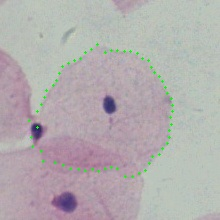
\includegraphics[width=0.3\textwidth]{00155origin.jpg}}
\hspace{0.01\textwidth}
\subfigure[插值点示意图]{\label{inserta:b}
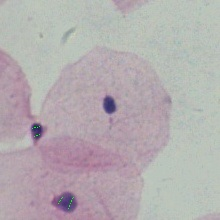
\includegraphics[width=0.3\textwidth]{00155RemoveP.jpg}}
\hspace{0.01\textwidth}
\subfigure[插值后结果]{\label{inserta:c}
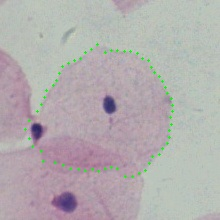
\includegraphics[width=0.3\textwidth]{00155Remove.jpg}}
\caption{插值处理前后结果对比图一}
\label{inserta}
\end{figure}

\begin{figure}[H]
\centering 
\subfigure[插值前结果]{\label{insertb:a}
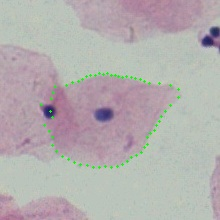
\includegraphics[width=0.3\textwidth]{00173origin.jpg}}
\hspace{0.01\textwidth}
\subfigure[插值点示意图]{\label{insertb:b}
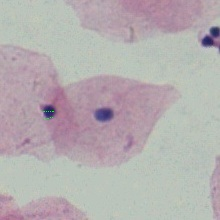
\includegraphics[width=0.3\textwidth]{00173RemoveP.jpg}}
\hspace{0.01\textwidth}
\subfigure[插值后结果]{\label{insertb:c}
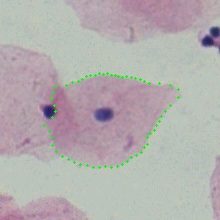
\includegraphics[width=0.3\textwidth]{00173Remove.jpg}}
\caption{插值处理前后结果对比图二}
\label{insertb}
\end{figure}



通过观察实验的样本图像,发现细胞核与细胞质相接区域往往具有较高的亮度,其亮度甚至可以与背景亮度相当,这可能是染色过程或成像设备造成的。在算法计算过程中这部分区域内采样点的梯度较大,代价较小,路径搜索过程中有被判断为细胞质边界点的可能性,会影响位于这些区域内采样点是否为边界点的判断。在提取细胞边界之前需要对这些区域进行处理,避免其对算法的准确度造成不良影响。为了解决这个问题,这里将细胞核及其附近高亮区域的代价设定为一个较大数值,使得算法将这里的采样点判断为边界的可能性几乎为零,有效的避免了将高亮区域判断为背景从而影响细胞质的分割结果。

\begin{figure}[H]
\centering 
\subfigure[优化高亮区域前结果]{\label{fig:subfig:a}
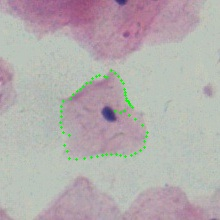
\includegraphics[width=0.3\textwidth]{00043BeforeLocalNur.jpg}}
\hspace{0.02\textwidth}
\subfigure[优化高亮区域后结果]{\label{fig:subfig:b}
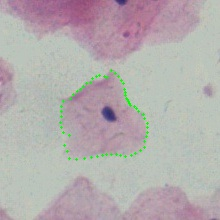
\includegraphics[width=0.3\textwidth]{00043LocalNur.jpg}}
\caption{高亮区域优化前后结果对比图}
\label{LocalNur}
\end{figure}

图\ref{LocalNur}(a)是最小代价路径算法的实验结果,从图\ref{LocalNur}(a)中明显看出有部分边界点受到细胞核与细胞质相接区域高亮像素点的影响,导致分割结果向细胞核靠近而产生不合理的分割效果,算法生成的边界路径在细胞质内部。图\ref{LocalNur}(b)为修正代价矩阵后的分割结果,通过算法求得的路径点接近真实的细胞质边界,有效地避免了细胞核与细胞质相接区域高亮像素点的干扰。

通过观察分析样本图像提取背景的颜色信息可知位于背景的像素在BGR三个通道都具有较高的值,很容易与其它非背景部分区分。在极坐标下得到的采样点,如果根据颜色及亮度某点$I\left ( r_{s},\theta _{j} \right )$被判定为背景像素,则推断出点$\left ( r_{i},\theta _{j} \right ),i\geq s$均不可能为当前细胞的细胞质边界点。因此,可对落在背景上的采样点相应位置的代价矩阵中的值进行设定,使得这些点被判断为细胞质边界的可能性几乎为零,提高算法的准确性。通过设置合适的阈值对实验图像进行背景的搜索,把判断为背景区域内的采样点相应的代价值设定为较大数值,使得最终分割结果的路径点不会分布在背景区域。


\begin{figure}[H]
\centering 
\subfigure[优化背景区域前结果]{\label{fig:subfig:a}
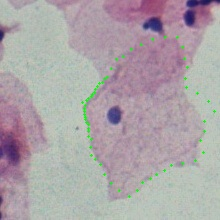
\includegraphics[width=0.3\textwidth]{00080beforeModify.jpg}}
\hspace{0.01\textwidth}
\subfigure[判断背景搜索线示意图]{\label{fig:subfig:b}
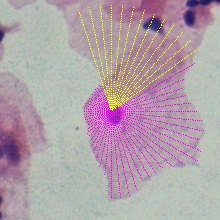
\includegraphics[width=0.3\textwidth]{00080.jpg}}
\hspace{0.01\textwidth}
\subfigure[优化背景区域后结果]{\label{fig:subfig:c}
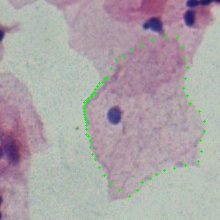
\includegraphics[width=0.3\textwidth]{00080Modify.jpg}}
\caption{优化背景区域前后结果对比图一}
\label{backgrounda}
\end{figure}

\begin{figure}[H]
\centering 
\subfigure[优化背景区域前结果]{\label{fig:subfig:a}
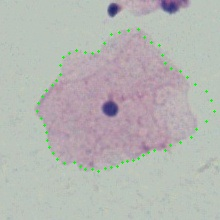
\includegraphics[width=0.3\textwidth]{00522beforeModify.jpg}}
\hspace{0.01\textwidth}
\subfigure[判断背景搜索线示意图]{\label{fig:subfig:b}
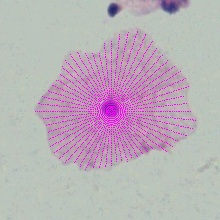
\includegraphics[width=0.3\textwidth]{00522.jpg}}
\hspace{0.01\textwidth}
\subfigure[优化背景区域后结果]{\label{fig:subfig:c}
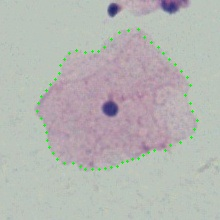
\includegraphics[width=0.3\textwidth]{00522Modify.jpg}}
\caption{优化背景区域前后结果对比图二}
\label{backgroundb}
\end{figure}

图\ref{backgrounda}(a)、图\ref{backgroundb}(a)是优化背景区域前的实验结果,观察可知部分路径点的位置分布在背景上,这些点与真实的细胞质边界有很大的偏差。如果把背景区域范围内的采样点都设置成不可能的路径点,那么最终的分割结果就不会有路径点分布在背景上,可以提升算法的分割效果。这里的搜索是对采样点进行的,搜索结果如图\ref{backgrounda}(b)、图\ref{backgroundb}(b)所示,紫色搜索线表示搜索到背景后停止搜索,黄色搜索线表示在采样范围内没有搜索到背景,实验结果表明背景区域内的采样点可以被准确地找到,便于下一步的优化。图\ref{backgrounda}(c)、图\ref{backgroundb}(c)是对背景区域进行优化后的实验结果,实验结果表明最终的路径点没有落在背景区域,分割效果得到有效提升。

不同$M$、$N$的分割效果对比图如图\ref{MN}所示。$M$的值表示分割结果中路径点的个数,$M$的值由小到大,则分割结果的路径点由少变多,分割效果越来越好。$N$的值表示个方向上采样点个数,$M$由小到大,每个采样方向上的采样点由稀疏变密集,分割效果越来越好。而$M$、$N$越大,则算法的采样点越多计算量越大,当$M=60$,$N=60$时,已获得达到良好的分割效果,因此本文算法中取$M=60$,$N=60$。

\begin{figure}[H]
\centering 
\subfigure[$M=20,N=60$]{\label{weight:a}
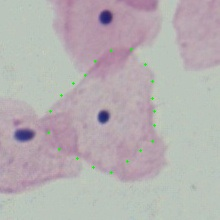
\includegraphics[width=0.3\textwidth]{p20-60.jpg}}
\hspace{0.01\textwidth}
\subfigure[$M=40,N=60$]{\label{weight:b}
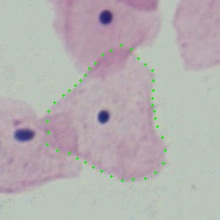
\includegraphics[width=0.3\textwidth]{p40-60.jpg}}
\hspace{0.01\textwidth}
\subfigure[$M=60,N=60$]{\label{weight:c}
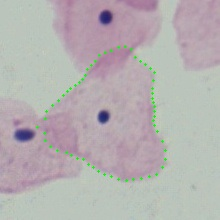
\includegraphics[width=0.3\textwidth]{p60-60.jpg}}
\vfill
\centering 
\subfigure[$M=60,N=20$]{\label{weight:d}
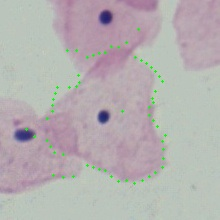
\includegraphics[width=0.3\textwidth]{p60-20.jpg}}
\hspace{0.01\textwidth}
\subfigure[$M=60,N=40$]{\label{weight:e}
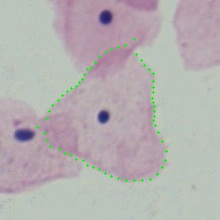
\includegraphics[width=0.3\textwidth]{p60-40.jpg}}
\hspace{0.01\textwidth}
\subfigure[$M=60,N=80$]{\label{weight:e}
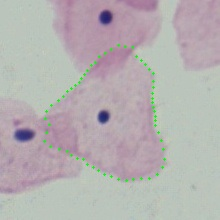
\includegraphics[width=0.3\textwidth]{p60-80.jpg}}
\caption{不同$M$、$N$分割效果对比图}
\label{MN}
\end{figure}

惩罚函数的系数对分割结果的影响如图\ref{weight}所示,其中图\ref{weight}(a)为原始图像,图\ref{weight}(b)、图\ref{weight}(c)、图\ref{weight}(d)、图\ref{weight}(e)、图\ref{weight}(f)依次为逐渐增大惩罚系数的分割结果。从实验结果可以看出,惩罚系数较小时,分割结果中大部分路径点都靠近细胞质的真实边界,少数路径点因受细胞质内部纹理干扰使分割结果产生陡峭的边界,偏离真实的细胞质边界。随着惩罚系数的增大,分割结果开始变得平滑,渐渐接近真实的细胞质边界。而当惩罚系数增大到一定程度后,分割结果会向圆形的趋势发展,导致分割结果严重偏离真实的细胞质边界。

\begin{figure}[H]
\centering 
\subfigure[原始图像]{\label{weight:a}
\includegraphics[width=0.3\textwidth]{00004-0Cy.jpg}}
\hspace{0.01\textwidth}
\subfigure[$\alpha=1.0,\beta=1.0,\gamma=1.0,\eta=1.0,\omega=1.0$]{\label{weight:b}
\includegraphics[width=0.3\textwidth]{00004-0c_2_Cy.jpg}}
\hspace{0.01\textwidth}
\subfigure[$\alpha=1.02,\beta=1.05,\gamma=1.1,\eta=1.5,\omega=2.0$]{\label{weight:c}
\includegraphics[width=0.3\textwidth]{00004-0c_7_Cy.jpg}}
\vfill
\centering 
\subfigure[$\alpha=1.1,\beta=1.5,\gamma=2.0,\eta=4.0,\omega=8.0$]{\label{weight:d}
\includegraphics[width=0.3\textwidth]{00004-0c_9_Cy.jpg}}
\hspace{0.01\textwidth}
\subfigure[$\alpha=1.1,\beta=1.6,\gamma=3.0,\eta=6.0,\omega=12.0$]{\label{weight:e}
\includegraphics[width=0.3\textwidth]{00004-0c_10_Cy.jpg}}
\hspace{0.01\textwidth}
\subfigure[$\alpha=3.0,\beta=6.0,\gamma=12.0,\eta=24.0,\omega=48.0$]{\label{weight:e}
\includegraphics[width=0.3\textwidth]{00004-0c_11_Cy.jpg}}
\caption{不同惩罚系数分割效果对比图}
\label{weight}
\end{figure}

为了避免分割结果出现陡峭的边界,算法限制了计算相邻两个路径点时在采样矩阵上列坐标的偏移,图\ref{Dis}是独立细胞不同列坐标偏移$d_{max}$情况下的实验结果。其中图\ref{Dis}(a)为原始图像,图\ref{Dis}(b)、图\ref{Dis}(c)、图\ref{Dis}(d)、图\ref{Dis}(e)、图\ref{Dis}(f)依次为逐渐增大$d_{max}$的分割结果。从实验结果可以看出,当允许的最大偏移等于0时表示路径上相邻两点在采样矩阵上列坐标一致,表现在极坐标下图像的分割结果就是路径点是距离极坐标原点距离相等的圆形。随着允许的最大偏移逐渐增大,路径点开始向真实的细胞质边界靠近。当$d_{max}=5$时,基本可以达到良好的分割效果。当$d_{max}=8$时,图\ref{Dis}(f)中分割结果的部分路径点之间距离发生较大改变,使得在陡峭的细胞质边界处分割效果得到改善。图\ref{Dis:h}~图\ref{Dis:l}是图\ref{Dis:g}重叠细胞不同列坐标偏移$d_{max}$情况下的实验结果。从图\ref{Dis:l}可以明显看出当$d_{max}=8$时,当前细胞分割结果的部分路径点会发生比较大的跳跃现象,而$d_{max}$值较小时路径点因受到约束而比较平滑,更符合细胞质边界的形态。实验结果表明较小的$d_{max}$会使分割结果受约束条件影响而过于接近圆弧形状,较大的$d_{max}$虽然会使分割结果在陡峭的边界处效果有所改善,但也可能导致路径点会发生不合理的跳跃现象,而且会加大算法的计算量。因此本文算法中选择$d_{max}=5$以获得较好的分割结果。

\begin{figure}[H]
\centering 
\subfigure[原始图像]{\label{Dis:a}
\includegraphics[width=0.3\textwidth]{27.jpg}}
\hspace{0.01\textwidth}
\subfigure[$d_{max}=0$]{\label{Dis:b}
\includegraphics[width=0.3\textwidth]{00027d0.jpg}}
\hspace{0.01\textwidth}
\subfigure[$d_{max}=1$]{\label{Dis:c}
\includegraphics[width=0.3\textwidth]{00027d1.jpg}}
\vfill
\centering 
\subfigure[$d_{max}=2$]{\label{Dis:d}
\includegraphics[width=0.3\textwidth]{00027d2.jpg}}
\hspace{0.01\textwidth}
\subfigure[$d_{max}=5$]{\label{Dis:e}
\includegraphics[width=0.3\textwidth]{00027d5.jpg}}
\hspace{0.01\textwidth}
\subfigure[$d_{max}=8$]{\label{Dis:f}
\includegraphics[width=0.3\textwidth]{00027d8.jpg}}
\vfill
\centering 
\subfigure[原始图像]{\label{Dis:g}
\includegraphics[width=0.3\textwidth]{74.jpg}}
\hspace{0.01\textwidth}
\subfigure[$d_{max}=0$]{\label{Dis:h}
\includegraphics[width=0.3\textwidth]{00074d0.jpg}}
\hspace{0.01\textwidth}
\subfigure[$d_{max}=1$]{\label{Dis:i}
\includegraphics[width=0.3\textwidth]{00074d1.jpg}}
\vfill
\centering 
\subfigure[$d_{max}=2$]{\label{Dis:j}
\includegraphics[width=0.3\textwidth]{00074d2.jpg}}
\hspace{0.01\textwidth}
\subfigure[$d_{max}=5$]{\label{Dis:k}
\includegraphics[width=0.3\textwidth]{00074d5.jpg}}
\hspace{0.01\textwidth}
\subfigure[$d_{max}=8$]{\label{Dis:l}
\includegraphics[width=0.3\textwidth]{00074d8.jpg}}
\caption{不同$d_{max}$分割效果对比图}
\label{Dis}
\end{figure}



优化修正后完整的最小代价路径算法流程如图\ref{MCPalgo}所示。

\begin{figure}[H]
\centering
\includegraphics[width=.36\textwidth]{MCPalgo.jpg}
\caption{最小代价路径算法流程图\label{MCPalgo}}
\end{figure}

相比许多形变模型在求解中只能求取局部最优解,本算法通过对图像进行适当的采样缩小了解空间,大大减少了计算量,因此可以快速求出全局最优解。
%对于$M\times N$的代价矩阵,穷举所有可能的路径共有$M^{N}$种可能,直接计算是不现实的。借鉴动态规划的思想,将最小代价路径的计算逐步分解成相邻两位置的代价计算,可以实现$O\left ( M^{2}N \right )$的时间复杂度。

%最终算法结果独立细胞 重叠细胞
\section{本章小结}
本章主要内容为最小代价路径算法,分采样模型的建立、代价矩阵的计算、最小代价路径的搜索等几部分进行阐述。

引言部分简要介绍了本文实验图片和细胞分割存在的问题难点。通过滤波实验结果对比了高斯滤波、均值滤波、中值滤波、双边滤波几种滤波方法对本论文实验图片的滤波效果,分析后选择中值滤波作为细胞图像的滤波处理方法。在分析了细胞质的形状颜色位置等特点后,采用了极坐标的方式建立采样模型从而得到采样矩阵,采样矩阵中记录了采样点红色通道绿色通道的差。

为了计算最小代价路径定义了代价矩阵,代价值的计算方法为利用同一采样方向上前后相邻的采样点的梯度差通过转换函数计算得出。然后,在代价矩阵的基础上介绍了最小代价路径的搜索方法,在路径点的搜索过程中添加了约束条件使得分割结果尽可能的趋于真实的细胞质边界。

通过分析实验结果中存在的相邻或重叠细胞核和当前细胞核附近高亮区域分割结果不合理,以及路径点落在背景而不是细胞质边界等问题,提出对算法的优化方法,即对采样矩阵和代价矩阵修正优化。实验结果表明优化后的最小代价路径算法对独立细胞和重叠细胞都有令人满意的分割效果,验证了算法的有效性。调整算法惩罚函数、坐标偏移参数得到不同参数下的分割结果,分析总结后为算法选取合适的参数。

最后,总结给出完整的最小代价路径算法。

\chapter{结合超像素的最小代价路径算法}

\section{引言}
计算机视觉领域有许多应用得益于超像素知识的深入研究发展。超像素的概念最早由Ren和Malik\cite{Ren2003Learning}提出的,超像素即将具有相似纹理、颜色、亮度等特征的相邻像素进行分组得到的形状不规则图像块。并指出好的分割应从相似性、邻近性和连续性等方面来评判,利用区域内和区域间的纹理相似性、亮度相似性、曲线连续性、以及轮廓能量四方面的特征对分割质量做评价。数字图像是由离散的像素点组成的,单个像素点对人类视觉来说没有直观的意义,而这些面积较小的、紧凑度强的、相似度高的像素集合一定程度上能够表达局部图像的结构特征。超像素分割处理的目的是把图像过分割成具有均匀视觉效果的小块紧凑区域。超像素在图像分割领域应用广泛,已发展为一种应用在图像预处理阶段的一项关键技术。

% \begin{figure}[H]
% \centering 
% \subfigure[原始图像]{\label{SPC:a}
% \includegraphics[width=0.45\textwidth]{SPC.jpg}}
% \hspace{0.01\textwidth}
% \subfigure[超像素分割结果]{\label{SPC:b}
% \includegraphics[width=0.45\textwidth]{retSPC.jpg}}
% \caption{超像素分割示意图}
% \label{SPC}
% \end{figure}

% 图\ref{SPC}展示了对彩色图像进行超像素分割后的结果,其中图\ref{SPC:a}是原始的彩色图像,图\ref{SPC:b}是超像素分割后的图像。从图\ref{SPC:b}可看出,超像素的数目远小于像素的数目,超像素的部分边界与分割目标的边界紧密贴合,在边界处的分割效果理想。可以利用分割得到的超像素边界提取分割目标的边界。
对彩色图像进行超像素分割后,超像素的数目远小于像素的数目,超像素的部分边界与分割目标的边界紧密贴合,在边界处的分割效果理想。可以利用分割得到的超像素边界提取分割目标的边界。本章主要介绍LRW算法、SLIC算法、SEEDS算法,并对超像素个数取不同值的分割结果进行分析,提出结合超像素方法的最小代价路径算法。

\section{超像素分割算法}

\subsection{LRW算法}
传统的RW算法是一种交互式的图像分割方法,给定一部分标记像素后,从未标记的像素开始随机漫步得到首次到达任一标记像素的概率,从而把未标记像素归类于最大概率相应的类标签。该算法的分割结果由未标记像素和最大到达概率的像素点之间的局部关系决定,忽略了未标记像素和其他标记像素的全局关系,可能会导致超像素结果形状不规则。Shen等人认为理想的超像素分割算法不仅能够使超像素的边界要和图像中目标的边界贴合,而且要保持复杂纹理区域的紧凑性约束。因此在RW算法的基础上提出了用于超像素的分割的LRW算法,并进行优化获得了良好的分割效果。

LRW算法\cite{Shen2014Lazy}包括两个重要的步骤,懒惰随机漫步与能量优化,前者通过在传统随机游走算法中添加顶点的自循环以获得懒惰性,能够充分地利用像素和种子点的全局关系,不断更新全局概率图和漫步时间策略,使得算法在微弱边缘和复杂的纹理区域界上具有更好的表现。而能量优化过程是为了避免算法受初始种子点的影响建立了一个能量优化框架,初始的超像素将利用一种能量函数被迭代地优化。优化策略本质上紧凑性约束,保证生成的超像素大小相近像素均匀。能量函数由两部分组成:一部分自适应地优化种子点的位置,使得超像素的边界靠近目标的边界;另一部分自适应性地把面积较大的超像素进行划分,使得超像素大小均匀。在优化的过程中更新了部分种子点的位置,同时因分割超像素出现了新的种子点,再次执行算法更新超像素分割结果。通过重新定位超像素的中心点,使用优化算法分割面积较大的超像素,改善了算法的分割效果。

最终的LRW算法流程如下:

输入:待分割图像I,初始种子点个数K,迭代次数T。

步骤1. 将K个种子点均匀的分布在图像I中。

步骤2. 使用懒惰随机游走调整初始种子点的位置。

步骤3. 计算最优化的能量E来修正超像素中心或将超像素分裂为2个。

步骤4. 使用懒惰随机游走更新每个像素所属的超像素以及超像素的中心。

步骤5. 若达到迭代次数T则算法结束,否则回到步骤3。

输出:超像素分割结果。



\begin{figure}[H]
\centering 
\subfigure[原始图像]{\label{LRW:a}
\includegraphics[width=0.3\textwidth]{107.jpg}}
\hspace{0.01\textwidth}
\subfigure[K=50]{\label{LRW:b}
\includegraphics[width=0.3\textwidth]{LRW50-107.jpg}}
\hspace{0.01\textwidth}
\subfigure[K=100]{\label{LRW:c}
\includegraphics[width=0.3\textwidth]{LRW100-107.jpg}}
\vfill
\centering 
\subfigure[K=250]{\label{LRW:d}
\includegraphics[width=0.3\textwidth]{LRW250-107.jpg}}
\hspace{0.01\textwidth} 
\subfigure[K=350]{\label{LRW:e}
\includegraphics[width=0.3\textwidth]{LRW350-107.jpg}}
\hspace{0.01\textwidth}
\subfigure[K=450]{\label{LRW:f}
\includegraphics[width=0.3\textwidth]{LRW450-107.jpg}}
\caption{LRW算法不同$K$值超像素分割结果}
\label{LRW}
\end{figure}

\begin{table}[H]
\centering
\caption{LRW算法不同$K$值超像素分割时间\label{LRWtime}}
\begin{tabular}{|p{2cm}<{\centering}|p{2cm}<{\centering}|p{2cm}<{\centering}|p{2cm}<{\centering}|p{2cm}<{\centering}|p{2cm}<{\centering}|}
\hline
 & K=50 & K=100 & K=250 & K=350 & K=450\\
\hline
时间(ms) & 175 & 295 & 330 & 375 & 482\\
\hline
\end{tabular}
\end{table}

LRW算法不同超像素个数分割结果如图\ref{LRW}所示。图\ref{LRW:a}为原始图像,图\ref{LRW:b}、图\ref{LRW:c}、图\ref{LRW:d}、图\ref{LRW:e}、图\ref{LRW:f}分别为超像素个数是50、100、250、350、450时的超像素分割结果。图\ref{LRW:b}的单个超像素面积较大,只有少部分超像素的边界接近真实的细胞质的边界,大部分超像素的边界与细胞质的边界有较大偏差,每个超像素内的颜色均一性较差。继续加大超像素个数以便获取更精确的分割结果,更有利于后续实验处理。当超像素个数逐渐增大,超像素的边界与真实的细胞质边界越接近,每个超像素的颜色更均一。当超像素个数为450时如图\ref{LRW:f}所示,超像素分割结果已经非常精细了。实验使用的计算机配置为Core2@2.66GHz,在VS2015环境下每张图像处理时间如表\ref{LRWtime}所示。虽然超像素的数目越多分割结果越准确,但是LRW算法运行速度缓慢,超像素个数越多运行时间越长,难以满足实际应用。



\subsection{SLIC算法}
在充分理解已有超像素分割算法的前提下,Achanta等人\cite{Achanta2012SLIC}认为满足实际需求的理想的方法须考虑以下几点内容:超像素的边界和图像中的边界几乎重合;在图像预处理阶段应用时,超像素应当被快速地计算出,具有高效的存储、易于使用的特性;当用于图像分割,超像素应同时提升分割结果的计算速度并改善其质量。随后提出了SLIC算法,主要采用将K-means方法在分割的过程中逐步迭代有效地生成超像素。并通过实验证明该方法比先前的方法在边界的分割效果更佳,速度更快,存储效率更高。

该算法有以下两个特点:通过限制搜索空间的区域范围与超像素的大小成比例,可以显著减少距离计算的次数,将复杂度降低到与像素数目成线性关系,而与超像素数目无关;使用带权重的距离测度结合像素的颜色和邻近空间,同时控制超像素的尺寸和紧凑度。

CIELAB颜色空间中有L、A、B三个分量,其中分量L表示亮度,A表示从品红色到绿色之间的颜色,B表示黄色到蓝色之间的颜色。该算法将彩色图片先转换到CIELAB颜色空间,以便获取聚类中心的特征向量$\left [ L\ A\ B\ x\ y \right ]^{T} $,(x,y)表示像素的位置。接下来依据特征向量设定相应的度量标准,最后像素进行局部聚类直至超像素分割完毕。

接下来介绍SLIC算法的具体步骤。首先是初始化种子点,假设预先设定的超像素个数为K, 那么就有K个初始聚类中心。一幅图像有N个像素,分割为k个尺寸相同的规则网格,即超像素大小为N/K个像素,相邻网格间距为$S=\sqrt{N/K}$。需要注意的是,预计的超像素尺寸为$S\times S$。计算尺寸为3$\times$3的窗口邻域内所有像素点的梯度值,聚类中心设定为该邻域内梯度最小的位置。这样做有效地避免种子点落在梯度较大的边界上或者受噪声干扰而影响后续算法的最终效果。

接下来判断像素归属于哪个聚类中心。标准的K-means搜索图像中每个聚类中心到每个像素的距离,而SLIC把搜索的范围限制为大小为$2S\times 2S$的窗口内,聚类中心位于窗口的中心,如下图所示。由于SLIC的搜索范围不是整个图像而是有限范围,有效地降低了计算量,也使得运算复杂度和超像素的数目无关。SLIC算法的复杂度和图像中像素的个数成线性关系,表示为O(N)。

通过计算每个像素点和它距离最近的种子点的距离测度,为每个像素点分配类标签。距离测度包括两个要素,颜色度量和空间度量。在对每个聚类中心进行搜索时,计算当前聚类中心和它周围$2S\times 2S$窗口搜索范围内每个像素点之间的距离测度。距离测度计算方法如下:

\begin{equation}
d_{c}=\sqrt{(l_{j}-l_{i})^{2}+(a_{j}-a_{i})^{2}+(b_{j}-b_{i})^{2}}
\label{SLICdc}
\end{equation}

\begin{equation}
d_{s}=\sqrt{(x_{j}-x_{i})^{2}+(y_{j}-y_{i})^{2}}
\label{SLICds}
\end{equation}

\begin{equation}
D^{'}=\sqrt{(\frac{d_{c}}{N_{c}})^{2}+(\frac{d_{s}}{N_{s}})^{2}}
\label{SLICd}
\end{equation}

其中,$d_{c}$表示颜色度量,$d_{s}$表示空间度量,$N_{s}=S=\sqrt{N/K}$表示最大空间度量,$N_{c}$表示最大颜色度量。最大颜色度量$N_{c}$的大小会因图片不同和聚类不同有明显的变化,因此解决这个问题的方法是一个用常数m代替。综上所述,最终的距离测度D如下:

\begin{equation}
D=\sqrt{d_{c}^{2}+(\frac{d_{s}}{S})^{2}m^{2}}
\label{SLICD}
\end{equation}

根据搜索规则,每个像素会被多个种子点搜索到,规定每个像素的聚类中心为距离测度最小值对应的种子点。每当一个像素被关联到最近的聚类中心后,将为这个聚类中心所在的超像素更新聚类中心。计算属于该聚类中心所有像素的向量$V =\left [ L\ A\ B\ x \ y \right ]^{T} $的均值,并用它作为新的聚类中心。当残差收敛时,表示超像素分割结束。残差使用$L_{2}$范式计算得出,把向量各元素的平方和再开平方,即欧式距离:

\begin{equation}
\left \| V \right \|_{2}=\sqrt{\sum_{i}v_{i}^{2}}
\label{SLICerror}
\end{equation}

计算每个超像素新的聚类中心,从而计算新聚类中心和之前的聚类中心的残差。迭代运行算法中分配聚类中心和判断残差步骤直至残差收敛,停止算法得到超像素分割结果。事实上,Achanta等人通过实验发现大多数图像迭代运行算法十次就可获得满意的分割结果,并以此为据对算法进行调整。

SLIC算法不同超像素个数分割结果如图\ref{SLIC}所示。图\ref{SLIC:a}为原始图像,图\ref{SLIC:b}是超像素个数为50时的实验结果,此时每个超像素包含的像素较多,每个超像素内的颜色分布不均匀,形状差异较大。图\ref{SLIC:c}是超像素个数为100时的实验结果,因为增加了超像素个数,超像素开始变得颜色均匀且紧凑。图\ref{SLIC:d}、图\ref{SLIC:e}、图\ref{SLIC:f}依次为超像素个数等于250、350、450时的超像素分割结果。随着超像素个数逐渐增多,超像素的边界越接近真实的细胞质边界,同时超像素的颜色更均一、形状更规则。特别是在颜色均匀的背景区域,超像素的形状更加规则近似矩形。$K=450$时,细胞质边界部分的超像素分割结果已经可以满足细胞质分割的需求了,无需继续增加$K$的值。在实验环境下不同$K$值SLIC算法C++代码的运行时间如表\ref{SLICtime}所示。从实验结果整体看来SLIC算法超像素分割结果紧凑且形状规则大小均匀,运算速度较快,$K=450$时平均每张实验图像用时75ms,很好地体现了SLIC算法的特点。
\begin{figure}[H]
\centering 
\subfigure[原始图像]{\label{SLIC:a}
\includegraphics[width=0.3\textwidth]{107.jpg}}
\hspace{0.01\textwidth}
\subfigure[K=50]{\label{SLIC:b}
\includegraphics[width=0.3\textwidth]{107slic50.jpg}}
\hspace{0.01\textwidth} 
\subfigure[K=100]{\label{SLIC:c}
\includegraphics[width=0.3\textwidth]{107slic100.jpg}}
\vfill
\centering
\subfigure[K=250]{\label{SLIC:d}
\includegraphics[width=0.3\textwidth]{107slic250.jpg}}
\hspace{0.01\textwidth} 
\subfigure[K=350]{\label{SLIC:e}
\includegraphics[width=0.3\textwidth]{107slic350.jpg}}
\hspace{0.01\textwidth}
\subfigure[K=450]{\label{SLIC:f}
\includegraphics[width=0.3\textwidth]{107slic450.jpg}}
\caption{SLIC算法不同$K$值超像素分割结果}
\label{SLIC}
\end{figure}

\begin{table}[H]
\centering
\caption{SLIC算法不同$K$值超像素分割时间\label{SLICtime}}
\begin{tabular}{|p{2cm}<{\centering}|p{2cm}<{\centering}|p{2cm}<{\centering}|p{2cm}<{\centering}|p{2cm}<{\centering}|p{2cm}<{\centering}|}
\hline
 & K=50 & K=100 & K=250 & K=350 & K=450\\
\hline
时间(ms) & 45 & 50 & 56 & 62 & 75\\
\hline
\end{tabular}
\end{table}


\subsection{SEEDS算法}
为了使分割出的超像素颜色相近大小相似,超像素分割算法普遍通过函数构建复杂的优化方案在效率和性能之间权衡比较,运算代价大速度慢而难以进行实际应用。SEEDS算法借鉴了爬山算法,获得初始超像素后通过迭代地修正超像素边界并对超像素的形状进行约束得到最终分割结果。

SEEDS算法\cite{Bergh2012SEEDS}首先进行粗分割,把图像用规则的网格均匀分割,每一格图像块作为初始的超像素。然后定义了一个具有鲁棒性的快速能量函数,从初始的超像素开始不断地修正超像素的边界,使得超像素的彩色直方图之间具有较高的相似性,同时调整超像素的规整性。修正的过程中,超像素从规则的网格形状开始生长,超像素之间通过不断地交换边界上的像素修正边界。算法迭代运行的次数越多,计算得到的能量函数的结果数值越大,分割结果更准确。实验时可通过设定终止时间停止运行算法。

假设图像有N个像素,期望分割为K个超像素。图像分割为超像素后,像素与超像素之间的映射关系可表示为,

\begin{equation}
s:\left \{ 1,\cdots, N \right \}\rightarrow \left \{ 1,\cdots ,K \right \}
\label{SEEDSmap}
\end{equation}

若$s(i)=k$表示像素i所属的超像素为k$(k\in K)$。每一个超像素是由一组像素组成的,这里用$A_{k}$表示第k个超像素,则$A_{k}$包含属于第k个超像素里的所有像素。

\begin{equation}
A_{k}=\left \{ i:s(i)=k \right \}
\label{SEEDSAk}
\end{equation}

分割后的图像可以表示为集合$\left \{ A_{k} \right \}$。因一个像素只能归属于一个超像素,集合$\left \{ A_{k} \right \}$的元素之间严格互斥,任意两个不同的超像素之间的交集为空,即$A_{k}\cap A_{k}^{'}=\varnothing $。

通过定义一个能量函数$E(s)$来衡量超像素分割的效果,将分割问题转化为一个最优化问题,即通过求解$s_{*}$来得到最终分割结果:

\begin{equation}
s^{*}=arg \max_{s\in S}E(s)
\label{SEEDSs}
\end{equation}

其中能量函数E(s)的定义为颜色分布项H(S)与边界项G(s)之和:

\begin{equation}
E(s)=H(s)+\gamma G(s)
\label{SEEDSE}
\end{equation}

$H(s)$表示超像素之间颜色的相似程度。统计各超像素的直方图,当属于同一超像素的像素的颜色分布最集中时$H(s)$的值最大。$G(s)$表示超像素边界形状的先验项,可控制超像素的形状。可以根据对分割结果形状的主观期望进行选择。系数$\gamma$用来平衡两项之间的影响,取合适的常数代替。

SEEDS算法不同超像素个数分割结果如图\ref{SEEDS}所示。图\ref{SEEDS:a}为原始图像,图\ref{SEEDS:b}是超像素个数为50时的实验结果,可见由于超像素个数较少,超像素内包含的像素点颜色差异较大,超像素的形状也非常不规则。图\ref{SEEDS:c}、图\ref{SEEDS:d}、图\ref{SEEDS:e}、图\ref{SEEDS:f}依次为超像素个数等于100、250、350、450时的超像素分割结果。超像素个数越多,超像素分割结果在真实的细胞质边界位置效果越好。整体看来SEEDS算法分割结果每个超像素的颜色均一,形状差异较大,超像素边界较SLIC算法的分割结果平滑。在与SLIC算法相同实验环境下不同$K$值SEEDS算法C++代码的运行时间如表\ref{SEEDStime}所示。实验表明SEEDS算法的运算速度较快,$K=450$时平均每张实验图像仅用时17ms,明显比SLIC算法的速度要快。
\begin{figure}[H]
\centering 
\subfigure[原始图像]{\label{SEEDS:a}
\includegraphics[width=0.3\textwidth]{107.jpg}}
\hspace{0.01\textwidth}
\subfigure[K=50]{\label{SEEDS:b}
\includegraphics[width=0.3\textwidth]{107seeds50.jpg}}
\hspace{0.01\textwidth}
\subfigure[K=100]{\label{SEEDS:c}
\includegraphics[width=0.3\textwidth]{107seeds100.jpg}}
\vfill
\centering 
\subfigure[K=250]{\label{SEEDS:d}
\includegraphics[width=0.3\textwidth]{107seeds250.jpg}}
\hspace{0.01\textwidth}
\subfigure[K=350]{\label{SEEDS:e}
\includegraphics[width=0.3\textwidth]{107seeds350.jpg}}
\hspace{0.01\textwidth}
\subfigure[K=450]{\label{SEEDS:f}
\includegraphics[width=0.3\textwidth]{107seeds450.jpg}}
\caption{SEEDS算法不同$K$值超像素分割结果}
\label{SEEDS}
\end{figure}

\begin{table}[H]
\centering
\caption{SEEDS算法不同$K$值超像素分割时间\label{SEEDStime}}
\begin{tabular}{|p{2cm}<{\centering}|p{2cm}<{\centering}|p{2cm}<{\centering}|p{2cm}<{\centering}|p{2cm}<{\centering}|p{2cm}<{\centering}|}
\hline
 & K=50 & K=100 & K=250 & K=350 & K=450\\
\hline
时间(ms) & 8 & 10 & 12 & 14 & 17\\
\hline
\end{tabular}
\end{table}



\section{结合超像素的最小代价路径算法}
从LRW算法、SLIC算法、SEEDS算法在细胞图像上的分割结果可知,细胞质边附近的超像素边界与真实细胞质边界趋于一致,可以利用超像素边界的这一特点提取细胞质的边界。这里通过计算每个超像素内像素的均值,然后用均值替换该超像素内的所有像素值生成均值图,运用最小代价路径算法得到细胞质分割结果绘制到原始图像上,生成分割结果图。


在采样过程中,在极坐标下对均值图采样获取采样矩阵,采样点规模与之前相同。因为均值图是由颜色均一的超像素组成的,所以同一超像素内的采样点值相同,接下来生成梯度矩阵中,靠近超像素边界的采样点因同一采样方向上相邻采样点具有不同的采样值而梯度值非零,若某采样点与计算梯度值相关前后相邻的采样点都在同一超像素范围内,则该采样点梯度值为零。因此,经过转换函数生成的代价矩阵中只有靠近超像素边界的采样点代价值较小,而梯度值为零的采样点相应的代价值为1。即在相邻超像素的边界附近的采样位置的代价值较小,其成为细胞质分割结果路径点的可能性较大,这样通过搜索最小代价路径寻求细胞质边界的方法仍然适用,最终的路径点将集中在相邻的超像素之间。

\begin{figure}[H]
\centering 
\subfigure[LRW结合修改前MCP]{\label{minValue:a}
\includegraphics[width=0.3\textwidth]{2-450blrw.jpg}}
\hspace{0.01\textwidth}
\subfigure[LRW结合修改后MCP]{\label{minValue:b}
\includegraphics[width=0.3\textwidth]{2-450clrw.jpg}}
\hspace{0.01\textwidth}
\subfigure[SLIC结合修改前MCP]{\label{minValue:c}
\includegraphics[width=0.3\textwidth]{2slic-avgb.jpg}}
\vfill
\centering 
\subfigure[SLIC结合修改后MCP]{\label{minValue:d}
\includegraphics[width=0.3\textwidth]{2slic-avgc.jpg}}
\hspace{0.01\textwidth}
\subfigure[SEEDS结合修改前MCP]{\label{minValue:e}
\includegraphics[width=0.3\textwidth]{2seeds-avgb.jpg}}
\hspace{0.01\textwidth}
\subfigure[SEEDS结合修改后MCP]{\label{minValue:f}
\includegraphics[width=0.3\textwidth]{2seeds-avgc.jpg}}
\caption{算法修改前后分割效果对比图}
\label{minValue}
\end{figure}

然而,均值图带来了新的问题。由于相邻的超像素之间有明显的界限,在图像中可看作是细胞质区域的纹理。颜色差异较大的相邻超像素之间的界限对细胞质分割结果产生了不良影响,如图\ref{minValue:a}、图\ref{minValue:c}、图\ref{minValue:e}所示,须对算法进行修改来解决这一问题。为了避免超像素之间的界限带来的强纹理效应,这里采用的方法是分别计算原始细胞图像和均值图的代价矩阵,然后逐一比较同一采样点在两个代价矩阵中的值,取较小的值作为最终的代价值用于计算最小代价路径。图\ref{minValue:b}、图\ref{minValue:d}、图\ref{minValue:f}为修改算法后将各方法的分割结果绘制到均值图的实验结果,该实验结果表明该方法有效地改善了分割结果,提高了算法的准确度。



利用LRW算法、SLIC算法、SEEDS算法的超像素分割结果分别生成均值图,使用结合超像素的最小代价路径算法的实验结果如图\ref{NMCP}。图\ref{NMCP}中第二列图是在第一列分割结果图的基础上通过分别计算每一个超像素内部包含的所有像素的均值,然后用相应的数值替换该超像素内的像素值,而得到的纹理、颜色、亮度均一的超像素图像。第三列为第二列均值图的最小代价路径算法的分割结果。该实验结果表明结合LRW算法、SLIC算法、SEEDS算法的最小代价路径算法对图中重叠细胞的分割均取得出色的分割效果。



\begin{figure}[H]
\centering 
\subfigure[LRW算法分割结果]{\label{NMCP:a}
\includegraphics[width=0.3\textwidth]{LRW450-107.jpg}}
\hspace{0.01\textwidth}
\subfigure[均值图]{\label{NMCP:b}
\includegraphics[width=0.3\textwidth]{LRW107-450.jpg}}
\hspace{0.01\textwidth}
\subfigure[分割结果]{\label{NMCP:c}
\includegraphics[width=0.3\textwidth]{LRW107-450c.jpg}}
\vfill
\centering 
\subfigure[SLIC算法分割结果]{\label{NMCP:d}
\includegraphics[width=0.3\textwidth]{107slic450.jpg}}
\hspace{0.01\textwidth}
\subfigure[均值图]{\label{NMCP:e}
\includegraphics[width=0.3\textwidth]{107slic-avg.jpg}}
\hspace{0.01\textwidth}
\subfigure[分割结果]{\label{NMCP:f}
\includegraphics[width=0.3\textwidth]{107slic-avgd.jpg}}
\vfill
\centering 
\subfigure[SEEDS算法分割结果]{\label{NMCP:g}
\includegraphics[width=0.3\textwidth]{107seeds450.jpg}}
\hspace{0.01\textwidth}
\subfigure[均值图]{\label{NMCP:h}
\includegraphics[width=0.3\textwidth]{107seeds-avg.jpg}}
\hspace{0.01\textwidth}
\subfigure[分割结果]{\label{NMCP:i}
\includegraphics[width=0.3\textwidth]{107seeds-avgc.jpg}}
\caption{结合LRW算法、SLIC算法、SEEDS算法的最小代价路径算法分割效果对比图}
\label{NMCP}
\end{figure}

图\ref{mcptosp}为最小代价路径算法分割结果与结合LRW算法、SLIC算法、SEEDS算法的最小代价路径算法分割结果对比,观察实验结果可知结合超像素方法的最小代价路径算法能够有效避免细胞质中存在的强纹理对分割结果的影响,而且在对比度低的细胞质部分分割结果较好,分割效果明显提高。

\begin{figure}[H]
\centering 
\includegraphics[width=0.18\textwidth]{460mcp.jpg}
\hspace{0.001\textwidth}
\includegraphics[width=0.18\textwidth]{499mcp.jpg}
\hspace{0.001\textwidth}
\includegraphics[width=0.18\textwidth]{580mcp.jpg}
\hspace{0.001\textwidth}
\includegraphics[width=0.18\textwidth]{648mcp.jpg}
\hspace{0.001\textwidth}
\includegraphics[width=0.18\textwidth]{684mcp.jpg}
\vfill
\vspace{6pt}
\centering 
\includegraphics[width=0.18\textwidth]{460lrwd.jpg}
\hspace{0.001\textwidth}
\includegraphics[width=0.18\textwidth]{499lrwd.jpg}
\hspace{0.001\textwidth}
\includegraphics[width=0.18\textwidth]{580lrwd.jpg}
\hspace{0.001\textwidth}
\includegraphics[width=0.18\textwidth]{648lrwd.jpg}
\hspace{0.001\textwidth}
\includegraphics[width=0.18\textwidth]{684lrwd.jpg}
\vfill
\vspace{6pt}
\centering 
\includegraphics[width=0.18\textwidth]{460slic-avgd.jpg}
\hspace{0.001\textwidth}
\includegraphics[width=0.18\textwidth]{499slic-avgd.jpg}
\hspace{0.001\textwidth}
\includegraphics[width=0.18\textwidth]{580slic-avgd.jpg}
\hspace{0.001\textwidth}
\includegraphics[width=0.18\textwidth]{648slic-avgd.jpg}
\hspace{0.001\textwidth}
\includegraphics[width=0.18\textwidth]{684slic-avgd.jpg}
\vfill
\vspace{6pt}
\centering 
\includegraphics[width=0.18\textwidth]{460seeds-avgd.jpg}
\hspace{0.001\textwidth}
\includegraphics[width=0.18\textwidth]{499seeds-avgd.jpg}
\hspace{0.001\textwidth}
\includegraphics[width=0.18\textwidth]{580seeds-avgd.jpg}
\hspace{0.001\textwidth}
\includegraphics[width=0.18\textwidth]{648seeds-avgd.jpg}
\hspace{0.001\textwidth}
\includegraphics[width=0.18\textwidth]{684seeds-avgd.jpg}
\caption{本文各算法的重叠细胞分割结果对比(第一行为最小代价路径算法分割结果,第三行、第四行、第五行分别为结合LRW算法、SLIC算法、SEEDS算法的最小代价路径算法分割结果。)}
\label{mcptosp}
\end{figure}

\section{算法评价}
通过将算法实验结果进行数据处理计算量化评价指标,可以衡量算法的好坏。为了对第三章提出的最小代价路径算法,以及本章结合LRW算法、SLIC算法、SEEDS算法的最小代价路径算法的性能进行量化评价,本章将对以上各分割方法和第二章介绍的RGVF细胞分割方法、水平集细胞分割方法的实验结果计算评价图像分割质量常用的评价指标以及记录其运行时间,得到实验数据进而对比分析算法的有效性并衡量以上各方法的性能。

用于量化评价分析的指标需要通过实验所得分割结果与真实的细胞质边界数据进行计算获取。Ground Truth是指通过手动标记得到的理论值,用于和实验结果进行比较分析的参照图像。真实的细胞质边界可通过手动标记的方式获得,本章的评价使用的真实细胞质边界数据来自手动标记结果。为了衡量各算法对独立细胞和重叠细胞的分割效果,尤其是本文提出的算法对重叠细胞的分割效果,标记的Ground Truth图像分为独立细胞图像和重叠细胞图像两类。
\subsection{评价指标}
首先介绍混淆矩阵(如表\ref{confusionM}所示),主要用于比较真实分类结果和预测分类结果,列表示真实的分类情况,行表示预测的分类情况。

\begin{table}[H]
\centering
\caption{混淆矩阵\label{confusionM}}
\begin{tabular}{|p{2cm}<{\centering}|p{2cm}<{\centering}|p{4cm}<{\centering}|p{4cm}<{\centering}|}
\hline
\multicolumn{2}{|c|}{} & \multicolumn{2}{|c|}{真实类别}\\
\cline{3-4}
\multicolumn{2}{|c|}{}  & 正例 & 负例\\
\hline
预测 & 正例 & True Positives & False Positives\\
\cline{2-4}
类别 & 负例 & False Negatives & True Negatives\\
\hline
\end{tabular}
\end{table}
其中,TP(True Positives)为真正例,表示预测的正例是真实正例的个数;FP(False Positives)为假正例,表示预测结果中的正例是真实负例的个数;FN(False Negatives)为假负例,表示预测结果中的负例是真实正例的个数;TN(True Negatives)为真负例,表示预测结果中的负例是真实负例的个数。TP与FN的总和表示真实正例的总数目,FP与TN的总和表示真实负例的总数目。本论文中TP表示分类为当前细胞的正确像素个数,FP表示不属于当前细胞却错分为当前细胞的像素个数,FN表示未分类为当前细胞且属于当前细胞的像素个数,TN表示正确分类为不属于当前细胞的像素个数。

准确率precision和召回率recall是广泛用于评价分类结果质量的指标,可以在混淆矩阵的基础上计算其值。准确率表示预测的正例是真实正例的个数与预测的正例总数之比。召回率表示预测结果的正例的个数与真实正例总数之比。在本文中,准确率表示实验分割结果分类为当前细胞的像素中真实属于当前细胞的像素个数所占比例,召回率表示实验分割结果正确分类为当前细胞的像素个数与真实属于当前细胞的像素总数之比。准确率、召回率的计算方法分别如下:

\begin{equation}
precision=\frac{TP}{TP+FP}
\label{precision}
\end{equation}

\begin{equation}
recall=\frac{TP}{TP+FN}
\label{recall}
\end{equation}

本文涉及的细胞质分割方法的分割实验结果可看作是把图像像素分类为当前细胞和除当前细胞之外部分共两类,可以用二分类的评价指标评价各分类方法的效果。衡量二分类问题的常用评价指标有$F_{1}$分数($F_{1}$ Score)、Matthews相关系数(MCC),可通过混淆矩阵中的TP、FP、FN、TN值计算。$F_{1}$分数也是准确率和召回率的调和平均数。$F_{1}$分数、MCC的值分布范围为$[0,1]$区间内,其值越大表明相应的分类方法效果越好。$F_{1}$分数、MCC的计算方法分别为:

\begin{equation}
F_{1}=2\cdot \frac{precision\cdot recall}{precision+recall}=\frac{2TP}{2TP+FP+FN}
\label{F1}
\end{equation}

\begin{equation}
MCC=\frac{TP\times TN-FP\times FN}{\sqrt{(TP+FP)(TP+FN)(TN+FP)(TN+FN)}}
\label{MCC}
\end{equation}

\subsection{分割结果评价分析}

实验使用的计算机配置为Core2@2.66GHz,内存8.00GB,实验环境为VS2015和MatlabR2012b。本论文研究内容所用的实验图片共871个,从中选择200个图像手动标记作为Ground Truth,其中独立细胞50个,重叠细胞150个。利用手动标记的真实值图像,通过设置阈值可以获得当前细胞的二值化掩模图像,用于计算各评价指标。红色曲线内区域表示属于当前细胞的像素,红色曲线外区域表示所有非当前细胞的像素。
\begin{figure}[H]
\centering 
\includegraphics[width=0.18\textwidth]{52gcline.jpg}
\hspace{0.001\textwidth}
\includegraphics[width=0.18\textwidth]{61gcline.jpg}
\hspace{0.001\textwidth}
\includegraphics[width=0.18\textwidth]{140gcline.jpg}
\hspace{0.001\textwidth}
\includegraphics[width=0.18\textwidth]{187gcline.jpg}
\hspace{0.001\textwidth}
\includegraphics[width=0.18\textwidth]{194gcline.jpg}
\vfill
\vspace{6pt}
\centering 
\includegraphics[width=0.18\textwidth]{28gcline.jpg}
\hspace{0.001\textwidth}
\includegraphics[width=0.18\textwidth]{34gcline.jpg}
\hspace{0.001\textwidth}
\includegraphics[width=0.18\textwidth]{63gcline.jpg}
\hspace{0.001\textwidth}
\includegraphics[width=0.18\textwidth]{95gcline.jpg}
\hspace{0.001\textwidth}
\includegraphics[width=0.18\textwidth]{105gcline.jpg}
\vfill
\vspace{6pt}
\centering 
\includegraphics[width=0.18\textwidth]{88gcline.jpg}%11
\hspace{0.001\textwidth}
\includegraphics[width=0.18\textwidth]{57gcline.jpg}
\hspace{0.001\textwidth}
\includegraphics[width=0.18\textwidth]{107gcline.jpg}
\hspace{0.001\textwidth}
\includegraphics[width=0.18\textwidth]{147gcline.jpg}
\hspace{0.001\textwidth}
\includegraphics[width=0.18\textwidth]{130gcline.jpg}%201
\vfill
\vspace{6pt}
\centering 
\includegraphics[width=0.18\textwidth]{20gcline.jpg}
\hspace{0.001\textwidth}
\includegraphics[width=0.18\textwidth]{40gcline.jpg}
\hspace{0.001\textwidth}
\includegraphics[width=0.18\textwidth]{176gcline.jpg}
\hspace{0.001\textwidth}
\includegraphics[width=0.18\textwidth]{229gcline.jpg}
\hspace{0.001\textwidth}
\includegraphics[width=0.18\textwidth]{300gcline.jpg}
\caption{Ground Truth(第一行、第二行为标记后的独立细胞的Ground Truth,第三行、第四行为标记后的重叠细胞的Ground Truth。)}
\label{GT}
\end{figure}


\begin{figure}[H]
\centering 
\includegraphics[width=0.18\textwidth]{52gcline.jpg}
\hspace{0.001\textwidth}
\includegraphics[width=0.18\textwidth]{61gcline.jpg}
\hspace{0.001\textwidth}
\includegraphics[width=0.18\textwidth]{140gcline.jpg}
\hspace{0.001\textwidth}
\includegraphics[width=0.18\textwidth]{187gcline.jpg}
\hspace{0.001\textwidth}
\includegraphics[width=0.18\textwidth]{194gcline.jpg}
\vfill
\vspace{6pt}
\centering 
\includegraphics[width=0.18\textwidth]{52RGVFline.jpg}
\hspace{0.001\textwidth}
\includegraphics[width=0.18\textwidth]{61RGVFline.jpg}
\hspace{0.001\textwidth}
\includegraphics[width=0.18\textwidth]{140RGVFline.jpg}
\hspace{0.001\textwidth}
\includegraphics[width=0.18\textwidth]{187RGVFline.jpg}
\hspace{0.001\textwidth}
\includegraphics[width=0.18\textwidth]{194RGVFline.jpg}
\vfill
\vspace{6pt}
\centering 
\includegraphics[width=0.18\textwidth]{52lsline.jpg}
\hspace{0.001\textwidth}
\includegraphics[width=0.18\textwidth]{61LSline.jpg}
\hspace{0.001\textwidth}
\includegraphics[width=0.18\textwidth]{140LSline.jpg}
\hspace{0.001\textwidth}
\includegraphics[width=0.18\textwidth]{187LSline.jpg}
\hspace{0.001\textwidth}
\includegraphics[width=0.18\textwidth]{194LSline.jpg}
\vfill
\vspace{6pt}
\centering 
\includegraphics[width=0.18\textwidth]{52MCPline.jpg}
\hspace{0.001\textwidth}
\includegraphics[width=0.18\textwidth]{61MCPline.jpg}
\hspace{0.001\textwidth}
\includegraphics[width=0.18\textwidth]{140MCPline.jpg}
\hspace{0.001\textwidth}
\includegraphics[width=0.18\textwidth]{187MCPline.jpg}
\hspace{0.001\textwidth}
\includegraphics[width=0.18\textwidth]{194MCPline.jpg}
\vfill
\vspace{6pt}
\centering 
\includegraphics[width=0.18\textwidth]{52LRWline.jpg}
\hspace{0.001\textwidth}
\includegraphics[width=0.18\textwidth]{61LRWline.jpg}
\hspace{0.001\textwidth}
\includegraphics[width=0.18\textwidth]{140LRWline.jpg}
\hspace{0.001\textwidth}
\includegraphics[width=0.18\textwidth]{187LRWline.jpg}
\hspace{0.001\textwidth}
\includegraphics[width=0.18\textwidth]{194LRWline.jpg}
\vfill
\vspace{6pt}
\centering 
\includegraphics[width=0.18\textwidth]{52slicline.jpg}
\hspace{0.001\textwidth}
\includegraphics[width=0.18\textwidth]{61slicline.jpg}
\hspace{0.001\textwidth}
\includegraphics[width=0.18\textwidth]{140slicline.jpg}
\hspace{0.001\textwidth}
\includegraphics[width=0.18\textwidth]{187slicline.jpg}
\hspace{0.001\textwidth}
\includegraphics[width=0.18\textwidth]{194slicline.jpg}
\vfill
\vspace{6pt}
\centering 
\includegraphics[width=0.18\textwidth]{52seedsline.jpg}
\hspace{0.001\textwidth}
\includegraphics[width=0.18\textwidth]{61seedsline.jpg}
\hspace{0.001\textwidth}
\includegraphics[width=0.18\textwidth]{140seedsline.jpg}
\hspace{0.001\textwidth}
\includegraphics[width=0.18\textwidth]{187seedsline.jpg}
\hspace{0.001\textwidth}
\includegraphics[width=0.18\textwidth]{194seedsline.jpg}
\caption{各算法的独立细胞分割结果对比(第一行为Ground Truth图像,第二行为RGVF方法分割结果,第三行为水平集方法分割结果,第四行为最小代价路径算法分割结果,第五行、第六行、第七行依次为结合LRW算法、SLIC算法、SEEDS算法的最小代价路径算法分割结果。)}
\label{ret}
\end{figure}

\begin{figure}[H]
\centering 
\includegraphics[width=0.18\textwidth]{176gcline.jpg}%11
\hspace{0.001\textwidth}
\includegraphics[width=0.18\textwidth]{57gcline.jpg}
\hspace{0.001\textwidth}
\includegraphics[width=0.18\textwidth]{107gcline.jpg}
\hspace{0.001\textwidth}
\includegraphics[width=0.18\textwidth]{147gcline.jpg}
\hspace{0.001\textwidth}
\includegraphics[width=0.18\textwidth]{31gcline.jpg}%201
\vfill
\vspace{6pt}
\centering 
\includegraphics[width=0.18\textwidth]{176lsline.jpg}
\hspace{0.001\textwidth}
\includegraphics[width=0.18\textwidth]{57lsline.jpg}
\hspace{0.001\textwidth}
\includegraphics[width=0.18\textwidth]{107lsline.jpg}
\hspace{0.001\textwidth}
\includegraphics[width=0.18\textwidth]{147lsline.jpg}
\hspace{0.001\textwidth}
\includegraphics[width=0.18\textwidth]{31lsline.jpg}
\vfill
\vspace{6pt}
\centering 
\includegraphics[width=0.18\textwidth]{176mcpline.jpg}
\hspace{0.001\textwidth}
\includegraphics[width=0.18\textwidth]{57mcpline.jpg}
\hspace{0.001\textwidth}
\includegraphics[width=0.18\textwidth]{107mcpline.jpg}
\hspace{0.001\textwidth}
\includegraphics[width=0.18\textwidth]{147mcpline.jpg}
\hspace{0.001\textwidth}
\includegraphics[width=0.18\textwidth]{31mcpline.jpg}
\vfill
\vspace{6pt}
\centering 
\includegraphics[width=0.18\textwidth]{176LRWline.jpg}
\hspace{0.001\textwidth}
\includegraphics[width=0.18\textwidth]{57LRWline.jpg}
\hspace{0.001\textwidth}
\includegraphics[width=0.18\textwidth]{107LRWline.jpg}
\hspace{0.001\textwidth}
\includegraphics[width=0.18\textwidth]{147LRWline.jpg}
\hspace{0.001\textwidth}
\includegraphics[width=0.18\textwidth]{31LRWline.jpg}
\vfill
\vspace{6pt}
\centering 
\includegraphics[width=0.18\textwidth]{176slicline.jpg}
\hspace{0.001\textwidth}
\includegraphics[width=0.18\textwidth]{57slicline.jpg}
\hspace{0.001\textwidth}
\includegraphics[width=0.18\textwidth]{107slicline.jpg}
\hspace{0.001\textwidth}
\includegraphics[width=0.18\textwidth]{147slicline.jpg}
\hspace{0.001\textwidth}
\includegraphics[width=0.18\textwidth]{31slicline.jpg}
\vfill
\vspace{6pt}
\centering 
\includegraphics[width=0.18\textwidth]{176seedsline.jpg}
\hspace{0.001\textwidth}
\includegraphics[width=0.18\textwidth]{57seedsline.jpg}
\hspace{0.001\textwidth}
\includegraphics[width=0.18\textwidth]{107seedsline.jpg}
\hspace{0.001\textwidth}
\includegraphics[width=0.18\textwidth]{147seedsline.jpg}
\hspace{0.001\textwidth}
\includegraphics[width=0.18\textwidth]{31seedsline.jpg}
\caption{各算法的重叠细胞分割结果对比(第一行为Ground Truth图像,第二行为水平集方法分割结果,第三行为最小代价路径算法分割结果,第四行、第五行、第六行依次为结合LRW算法、SLIC算法、SEEDS算法的最小代价路径算法分割结果。)}
\label{ret2}
\end{figure}

本文提出方法的分割结果为一组路径点,为了便于分析将这些路径点连接起来作为分割结果,获取掩模用于评价指标的计算。实验中获取结合LRW算法、SLIC算法、SEEDS算法的最小代价路径算法的细胞质分割结果时,统一设定超像素个数为450。部分实验结果如图\ref{ret}、图\ref{ret2}所示,展示了最小代价路径算法、结合LRW算法、SLIC算法、SEEDS算法的最小代价路径算法以及RGVF方法、水平集方法的分割效果。由于RGVF方法只适用于分割独立细胞,这里仅给出其对独立细胞分割结果。

为了更具体的衡量算法解决重叠细胞分割问题的有效性,分别对独立细胞和重叠细胞的实验结果计算评价指标,如表\ref{One}、表\ref{Olap}所示,其中MCP表示最小代价路径算法。由于RGVF方法只适用于分割独立的细胞,这里只计算其分割独立细胞的评价指标。

\begin{table}[H]
\centering
\caption{独立细胞分割结果的评价指标\label{One}}
\begin{tabular}{|p{3cm}<{\centering}|p{2cm}<{\centering}|p{2cm}<{\centering}|p{2cm}<{\centering}|p{2cm}<{\centering}|}
\hline
算法 & precision & recall & $F_{1}$分数 & MCC \\
\hline
RGVF & 0.953746 & 0.963273 & 0.958486 & 0.946981 \\
\hline
Level Set & 0.807507 & 0.975671 & 0.883660 & 0.856569 \\
\hline
MCP & 0.959282 & 0.986164 & 0.972537 & 0.965525 \\
\hline
LRW+MCP & 0.977335 & 0.977584 & 0.977459 & 0.971875 \\
\hline
SLIC+MCP & 0.979057 & 0.974184 & 0.976615 & 0.970709 \\
\hline
SEEDS+MCP & 0.971755 & 0.980267 & 0.975993 & 0.969822 \\
\hline
\end{tabular}
\end{table}

\begin{table}[H]
\centering
\caption{重叠细胞分割结果的评价指标\label{Olap}}
\begin{tabular}{|p{3cm}<{\centering}|p{2cm}<{\centering}|p{2cm}<{\centering}|p{2cm}<{\centering}|p{2cm}<{\centering}|p{2cm}<{\centering}|}
\hline
算法 & precision & recall & $F_{1}$分数 & MCC \\
\hline
Level Set & 0.817070 & 0.950065 & 0.878563 & 0.838074 \\
\hline
MCP & 0.920301 & 0.945526 & 0.932743 & 0.909609 \\
\hline
LRW+MCP & 0.926726 & 0.965391 & 0.945664 & 0.934299 \\
\hline
SLIC+MCP & 0.928129 & 0.961562 & 0.944549 & 0.925629 \\
\hline
SEEDS+MCP & 0.928824 & 0.962404 & 0.945316 & 0.926661 \\
\hline
\end{tabular}
\end{table}

从表\ref{One}中可以看出RGVF细胞分割方法对独立细胞的分割效果良好。本文提出的分割算法对独立细胞分割的评价指标$F_{1}$分数和MCC都略高于RGVF细胞分割方法,说明本文提出的算法可以有效地分割独立细胞。而水平集细胞分割方法的准确率和 $F_{1}$分数明显低于其他几种方法。
从表\ref{Olap}中可以看出本文提出的分割算法对重叠细胞的分割均取得良好的效果,$F_{1}$分数和MCC值都明显大于水平集方法分割结果的相应指标。结合超像素的最小代价路径算法的$F_{1}$分数值均略高于原始的最小代价路径算法,同时MCC值明显高于最小代价路径算法,表明使用超像素分割方法提取细胞质的边界有利于提高最小代价路径算法的分割效果。另外,水平集方法对独立细胞、重叠细胞分割结果的召回率均明显高于准确率。
综合看来,结合超像素算法的最小代价路径算法分割评价指标优于最小代价路径算法,结合LRW算法的最小代价路径算法的评价指标均优于其他算法。


\begin{table}[H]
\centering
\caption{RGVF方法、水平集方法、最小代价路径算法平均运行时间\label{timeMatlab}}
\begin{tabular}{|p{2cm}<{\centering}|p{2cm}<{\centering}|p{2cm}<{\centering}|p{2cm}<{\centering}|}
\hline
算法 & RGVF & Level Set & MCP\\
\hline
时间(s) & 108.3 & 28.8 & 2.3\\
\hline
\end{tabular}
\end{table}

\begin{table}[H]
\centering
\caption{最小代价路径算法、结合LRW算法、SLIC算法、SEEDS算法的最小代价路径算法平均运行时间\label{timeC}}
\begin{tabular}{|p{2cm}<{\centering}|p{2.5cm}<{\centering}|p{2.5cm}<{\centering}|p{2.5cm}<{\centering}|p{2.5cm}<{\centering}|}
\hline
算法 & MCP & LRW+MCP & SLIC+MCP & SEEDS+MCP\\
\hline
时间(ms) & 17 & 498 & 92 & 35\\
\hline
\end{tabular}
\end{table}

表\ref{timeMatlab}中的时间是算法在MatlabR2012b环境下平均每个细胞的运行时间。
表\ref{timeC}中的时间是算法在VS2015环境下平均每个细胞的运行时间。结合超像素方法的最小代价路径算法由于增加了超像素分割的步骤其整体运行时间代价较大。综合比较各算法运行时间说明最小代价路径算法速度比RGVF方法、水平集方法快,同时比结合超像素方法的最小代价路径算法的运行时间快。

图\ref{retSumgood}展示了结合SEEDS算法的最小代价路径算法对重叠情况复杂宫颈细胞的分割结果,说明该方法能够有效解决重叠情况复杂细胞的分割问题。
\begin{figure}[H]
\centering 
\includegraphics[width=0.3\textwidth]{603seedsline.jpg}
\hspace{0.001\textwidth}
\includegraphics[width=0.3\textwidth]{625seedsline.jpg}
\hspace{0.001\textwidth}
\includegraphics[width=0.3\textwidth]{656seedsline.jpg}
\vfill
\vspace{6pt}
\centering 
\includegraphics[width=0.3\textwidth]{671seedsline.jpg}
\hspace{0.001\textwidth}
\includegraphics[width=0.3\textwidth]{747seedsline.jpg}
\hspace{0.001\textwidth}
\includegraphics[width=0.3\textwidth]{821seedsline.jpg}
\caption{重叠情况复杂的细胞分割结果}
\label{retSumgood}
\end{figure}

\section{本章小结}
本章主要内容为结合超像素的最小代价路径算法的研究和算法的评价。

首先,分别介绍了LRW算法、SLIC算法、SEEDS算法三种超像素分割方法的基本内容,给出不同超像素个数情况下的实验结果并进行对比分析。实验结果表明超像素个数取值越大细胞质边界上的超像素分割结果越准确,LRW算法、SLIC算法、SEEDS算法的运算速度依次由慢到快,LRW算法速度是SLIC算法、SEEDS算法的几十倍,难以满足实际应用。然后提出结合超像素分割结果的最小代价路径分割方法。具体方法是在超像素分割结果的基础上计算每一个超像素内像素的均值,替换属于同一超像素内的所有像素值,对替换后生成的图像运行最小代价路径算法得到细胞质分割结果并绘制到原始图像上,得到最终的分割结果。通过实验对比了结合LRW算法、SLIC算法、SEEDS算法的最小代价路径分割结果,验证了算法的有效性。

最后,对RGVF细胞分割方法、水平集细胞分割方法、最小代价路径算法,以及结合SLIC算法、SEEDS算法的最小代价路径算法的独立细胞和重叠细胞的分割结果进行量化评估,验证了本文提出算法的有效性。

\chapter{总结与展望}
\section{论文工作总结}
本文主要研究宫颈细胞分割问题,为计算机辅助诊断技术提供便利。

分析宫颈细胞图像特点后,提出了一种高效的自动分割细胞的方法最小代价路径算法。首先对细胞图像进行中值滤波,根据细胞质在图像中的形态、位置特点在极坐标下获取采样点,然后计算梯度矩阵并转换生成代价矩阵,添加边界约束条件之后搜索全局最小代价路径。针对实验结果出现的不合理分割结果进行分析并进一步完善算法,增加了修正优化处理步骤,实验结果表明该算法在独立细胞和重叠细胞图像上均取得良好的分割效果。

介绍了LRW算法、SLIC算法、SEEDS算法的基本原理,并通过实验结果对比分析了不同超像素个数情况下细胞图像的超像素分割结果,选择合适的超像素个数用于细胞质分割的研究。利用超像素分割结果与细胞质边界的关系,在超像素分割结果的基础上生成均值图,之后为了避免超像素间出现的强纹理对分割结果的影响修改最小代价路径算法,最终通过实验证明了算法的有效性。

为了衡量本文提出的细胞分割方法的效果,在分割结果的基础上获取掩模图像,使用二分类评价指标量化评价了最小代价路径算法,结合LRW算法、SLIC算法、SEEDS算法的最小代价路径算法,以及RGVF方法和水平集方法的分割结果,并对比了以上各方法的运行时间,实验数据说明本文提出的方法快速有效地解决了重叠细胞的分割问题。



\section{研究方向展望}
通过对大量细胞图像实验结果的评价分析,验证了本文提出的最小代价路径算法以及结合超像素分割方法的最小代价路径算法解决独立细胞和重叠细胞分割问题的有效性,同时具较高计速度能够满足宫颈刮片自动析的实际应用需求,但仍有可以改进的地方,可从以下几方面进一步研究探索:

利用采样矩阵计算梯度信息时,只简单地考虑了同一采样方向前后相邻的采样点信息,没有结合相邻采样方向上距离较近的采样点信息。可以考虑提取图像中采样点位置较近的多个采样点信息,构建更有利于细胞质分割的计算梯度值模型。

代价矩阵是最小代价路径算法的基础,因此寻求更佳的转换函数显得尤为重要。可以寻求采用更复杂的数学模型进行实验,使得位于真实细胞质边界的采样点代价值较其余部分的代价值更易于区分,提高续路径搜索结果的准确率。

在选择相邻路径点最大偏移参数时,本论文综合考虑实验结果选择最大偏移参数为5,导致一些细胞质边界较尖锐的区域真实相邻路径点偏移较大,而算法最终得到的路径点落在了细胞质内部而未能准确分割。需要针对尖锐细胞质边界错分割情况进行研究,提出更有效的边界约束条件来优化算法的分割结果。

由于扫描获取的宫颈刮片图像中部分细胞存在形状变化较大、褶皱严重、多个细胞大面积重叠等因素,本文提出的算法未能对这些情况复杂的图像给出满意的分割结果,只能根据算法的运行结果绘制出一条闭合曲线。如图\ref{retCon}所示为结合SEEDS的最小代价路径算法对重叠情况复杂的细胞分割结果。后续的研究工作应着力提高算法处理形变褶皱严重、重叠情况复杂的细胞图像的准确度。

\begin{figure}[H]
\centering 
\includegraphics[width=0.3\textwidth]{17seedsline.jpg}
\hspace{0.001\textwidth}
\includegraphics[width=0.3\textwidth]{36seedsline.jpg}
\hspace{0.001\textwidth}
\includegraphics[width=0.3\textwidth]{71seedsline.jpg}
\vfill
\vspace{6pt}
\centering 
\includegraphics[width=0.3\textwidth]{88seedsline.jpg}
\hspace{0.001\textwidth}
\includegraphics[width=0.3\textwidth]{106seedsline.jpg}
\hspace{0.001\textwidth}
\includegraphics[width=0.3\textwidth]{181seedsline.jpg}
\caption{重叠情况复杂的细胞分割结果}
\label{retCon}
\end{figure}



相比最小代价路径算法,结合超像素算法的最小代价路径算法的分割效果有所提升,但增加了算法整体的运行时间。为追求更快的处理时间,须对算法进行优化,或者寻求更快速有效的超像素分割方法,也可以结合其他能够提取到细胞质边界的算法进行实验研究。

\acknowledgement
斗转星移,四季更迭,转眼间我的研究生生活即将进入尾声。东南大学历史悠久、人才辈出,校园里的连绵的梧桐树、庄重典雅的大礼堂等都展示着学校深厚的文化底蕴。这三年的时间里我在东南大学不断地汲取养分,成长收获。在这里衷心地向所有关心我、支持我的人表示感谢,在他们的帮助下我顺利地完成课题研究并撰写此论文。

感谢我的导师舒华忠教授,舒老师治学严谨、学识渊博、关怀学生,深受大家的爱戴。感谢他认真仔细的批阅论文,对论文撰写给予详尽的指导。舒老师的一言一行都是我今后学习的榜样,再次向舒老师表示诚挚的谢意。

感谢我的指导老师王征,感谢他在课题研究期间给予我的帮助和指导。从研究方向的确定、论文的选题、研究过程中遇到的难题,王老师都不遗余力地提供指导和帮助。课题研究期间,王老师不仅带领我一起分析实验结果探讨问题的解决方案,还耗费大量时间帮助我完成了图像的手动标记。

感谢杨冠宇老师在研究课题期间给予的指导和帮助,针对我的研究内容提供了清晰的思路和建议,在他的帮助下课题研究进展顺利。

感谢实验室的所有同学在学习上给予我的帮助,在实验室一起学习讨论、友爱互助的氛围里,我收获了知识和友谊。愿他们事业顺利、前程似锦。

感谢舍友们给予我的陪伴和包容,这三年里一起分享喜悦,在同一屋檐下共同成长,她们的欢声笑语让我的生活充满生机与活力,愿她们今后的工作生活都一帆风顺。

感谢父母的养育之恩和家人一直以来默默的支持和帮助,他们给了我最大的支持和动力。远离家乡的我经常会思念家乡,特别是我的父母,每次通电话或者视频都能感受到他们的惦念和无微不至的关心。

最后,再次向所有在生活、学习中给予我关怀的人们表示感谢,衷心地祝福你们,祝福东南大学!


\thesisbib{seuthesix}
\end{document}
